\documentclass[conf]{new-aiaa}
%\documentclass[journal]{new-aiaa} for journal papers
\usepackage[utf8]{inputenc}

\usepackage{graphicx}
\usepackage{amsmath}
\usepackage[version=4]{mhchem}
\usepackage{siunitx}
\usepackage{subfig}
\usepackage{longtable,tabularx}
\setlength\LTleft{0pt} 
\usepackage[export]{adjustbox}
\usepackage{placeins}

\title{Benefits of Two Turbine Rotor Diameters and Hub Heights in the Same Wind Farm}

\author{Andrew PJ Stanley\footnote{PhD Candidate, Department of Mechanical Engineering, 435 CTB, AIAA Student Member.} and Andrew Ning\footnote{Assistant Professor, Department of Mechanical Engineering, 435 CTB, AIAA Senior Member.}}
\affil{Brigham Young University, Provo, Utah, 84602}
\author{Katherine Dykes\footnote{Senior Engineer, National Wind Technology Center, 18200 CO-128, Boulder, CO 80303.}}
\affil{National Renewable Energy Laboratory, Golden, Colorado, 80401}


\begin{document}

\maketitle

\begin{abstract}
Significant turbine-wake interactions greatly reduce power output in a wind farm. If different turbine hub heights and rotor diameters are included in the same wind farm, the wake interference in the farm will be reduced, resulting in a lower cost of energy (COE) than a farm with identical turbines. In this paper, we present a method to model wind farm COE in farms with hub heights and rotor diameters that vary across the wind farm. We also demonstrate how to optimize these wind farms to minimize COE. The results show that COE can be greatly reduced in wind farms with non-homogeneous turbines, especially when the turbines are spaced close together.
For a unidirectional wind rose, including different turbine design in the wind farm has a similar decrease in COE to spreading the wind turbines farther apart.
When the rotor diameter and hub height of the wind turbines in a farm are optimized uniformly, a COE decrease of 4\% to 13\% (depending on the grid spacing and wind shear exponent) is achieved compared to the baseline. When the rotor diameter and turbine heights are optimized non-uniformly, with two different diameters and heights throughout the farm, there is a COE decrease of 22\% to 41\% compared to the baseline. For a more spread wind rose with a dominant probability from the west, there is a COE decrease between 3\% and 10\% for uniformly optimized rotor diameter and height compared to the baseline. With two optimized rotor diameters and heights through the farm, a COE decrease of 3\% to 19\% is achieved. For a similar wind rose shifted such that the dominant wind direction is from the northwest, a COE decrease between 3\% and 10\% results from uniformly optimized wind turbines compared to the baseline. A COE decrease of 3\% to 17\% compared to the baseline occurs with two different turbines are optimized throughout the wind farm.
% For a unidirectional wind rose, the optimal COE in a closely spaced grid with two different turbine groups is better than a grid spaced much farther apart with only one turbine group.
% COE decreases between 19\% to 33\% from a uniform turbine wind farm to a farm with two different hub heights and rotor diameters throughout the farm. This COE decrease is for a unidirectional wind rose. Other wind distributions are also considered, for which this COE decrease varies between 1\% and 11\%.
% The COE decrease from one turbine group to two varies between 19\% and 33\% for a unidirectional wind rose across all the grid spacing and shear exponents analyzed. For other wind roses, the benefit varies from 1\% to 11\%, with the greatest benefit occurring at the smallest grid spacing. 
\end{abstract}

\section{Introduction}

Turbine-wake interactions in wind farms greatly reduce energy production, often by 10-20\% \cite{wakeLoss1,wakeLoss2}. Research has shown that wind farm layout optimization and yaw control can be used to minimize turbine-wake interactions and maximize energy production \cite{wagner2011optimizing,Fleming2015-Wind-Plant,Gebraad2015-Maximization-Annual}. In this paper we discuss another method to reduce wake interference; varying turbine design. Allowing turbine heights and rotor diameters to vary throughout the wind farm introduces an additional dimension that can be used to reduce wake effects in a wind farm, resulting in a lower cost of energy (COE).

Several studies have shown increased energy production and a decrease in COE for wind farms with non-homogeneous turbine heights. Chen et al.\ used two turbine designs, each with a different hub height  \cite{chen2013wind}. With a predetermined number of wind turbines, they used a genetic algorithm to optimize the layout and type of each turbine in the farm. When combining the different turbines in a farm, the optimal energy production increased by 13.53\%, and the COE decreased by 0.37\% compared to when only one turbine type was used. By using two predefined wind turbines, Chen et al.\ avoids the need to constrain the turbine structurally because each turbine is already fully designed.

In our previous research, we used gradients to optimize a wind farm while including the turbine hub height and tower design as variables  \cite{Stanley2017_WE}. The turbine hub height could vary freely, and the changing structural requirements from the height variation was accounted for by changing the tower diameter and shell thickness. We found that different hub heights are most beneficial in wind farms with low wind shear, small rotor diameters, and turbines that are close together. For many cases, the COE reduction was greater than 10\% when two different hub heights were used in a wind farm. However, even in less ideal cases, with turbines spaced farther apart or with high wind shears, different hub heights still resulted in a 2-3\% lower COE than when only one turbine height was used throughout the farm.

Hazra et al.\ optimized turbine rotor diameter, along with turbine height in a small farm \cite{HazraMMZ15}. Using a particle swarm method, they found that cost of power decreased by 12\% when the farm is optimized in three dimensions compared to a traditional two-dimensional optimization. In this research, they do not address the additional cost and structural requirements from taller towers and larger rotor diameters.

Like wind farm layout optimization and yaw control, optimizing turbine design in non-homogeneous turbine wind farms reduces COE. This research addresses wind farms with non-homogeneous turbine hub heights and rotor diameters. We used gradient-based optimization to allow our methodology to scale well for large wind farms with many design variables. Also, in addition to power variation, we account for the difference in cost from changing the tower height and rotor diameter. Finally, in this study we constrain the tower and rotor structurally to account for the variations in thrusts and moments from the changing turbine design.

\section{Methodology}

In this section, we discuss the models used for turbine wakes, wind and power calculation, rotor loads and mass, tower loads and mass, wind farm cost, and finally the optimization.

\subsection{Wake Model}
In this study, the FLORIS wake model is used to calculate wind speeds throughout the farm \cite{Gebraad-yaw-control}. A slightly modified version of the FLORIS wake model is used to account for three-dimensional variations in the wake \cite{stanley2017gradient}.

\subsection{Wind Model and Power Calculation}
To account for wind speed variations with height, we used a power law approximation.
\begin{equation}
	U(z) = U_{ref}\bigg(\frac{z}{z_{ref}}\bigg)^\alpha
    \label{shear}
\end{equation}
The reference wind speed, $U_{ref}$ is measured at the reference height, $z_{ref}=50$ meters. The shear exponent, $\alpha$, defines how fast the wind speed changes with height. A low shear is typical over open waters and flat fields without tall vegetation, while higher wind shear values are typical in rougher terrain such as cities and hilly areas. The hub speed, $U$, is thus calculated as a function of the hub height, $z$. 
In this study, power is calculated with the hub height wind speed. In addition, we use a constant power coefficient $C_P=0.42$, and a turbine rating of 5 megawatts.

\subsection{Rotor Model}
Because the rotor diameter varies in this study, there was a need to implement a rotor model to calculate the blade mass and loads as a function of rotor diameter. To accomplish this, we used RotorSE,  a rotor model based primarily on blade element momentum theory and beam finite element analysis developed at the National Renewable Energy Laboratory (NREL) \cite{ning2013rotorse}. RotorSE is a relatively complex model, and allows for a lot of freedom in rotor analysis. 

For this study, the only RotorSE input that changed was the rotor diameter. To speed up the optimization by eliminating the need to run RotorSE at every iteration of the optimization, we created a simple surrogate model from optimized RotorSE outputs as a function of the rotor diameter. We did a sweep of rotor diameters, and at each point minimized the blade mass with the chord and twist distributions as design variables. The $C_P$ was constrained to be greater than 0.42, and the blade was constrained structurally for strain, buckling, and first natural frequency. With this process, we created a fast and accurate relation between the rotor diameter and the structure and load values required in our system.
% By doing a sweep of this variable we extracted points from the RotorSE analysis and fit a function to the rotor diameter for each output of interest. At each RotorSE analysis point, the blade chord and twist distributions were optimized to ensure that the blade remained structurally sound at each rotor diameter. With this process, we created a fast and accurate relation between the rotor diameter and the structure and load values required in our system.

\subsection{Tower Model}
As the rotor diameter and tower heights change, it is necessary to adjust the tower such that it can support the required moments and loads. We modeled the tower as a tapered steel cylinder. As shown in Fig. \ref{tower_def}, the tower diameter and shell thickness were defined at the bottom, midpoint, and top of the tower, and were linearly interpolated in between.
\begin{figure}[htbp]
\centering
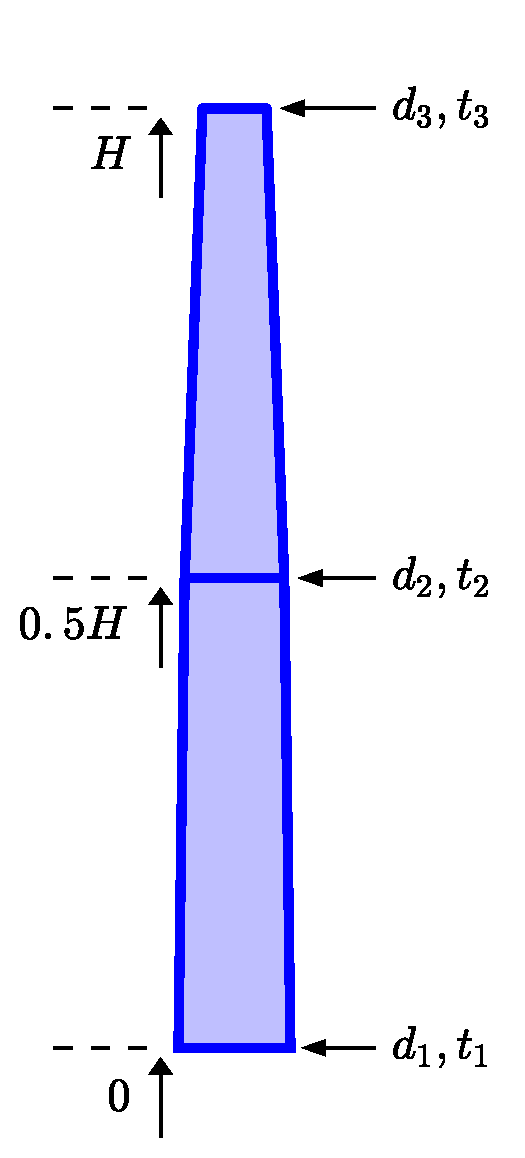
\includegraphics[width=.25\textwidth]{tower_param.pdf}
\caption{\label{tower_def}Parameterization of the wind turbine towers.}
\end{figure}
Using the mass, thrust, and torque calculated from the rotor model, the maximum stress and buckling values were computed along the length of the tower (both at the maximum thrust and maximum wind speed) using the method outlined in Eurocode \cite{eurocode3}.

We calculated the first natural frequency of the tower by approximating it as a cantilever beam with an end mass using the method described by Erturk et al \cite{erturk2011appendix}. Erturk's method assumes a constant diameter and mass distribution along the length of the beam, which is clearly not the case for a tapered tower. We averaged these values across the tower, and to account for any difference we compared our natural frequency calculation to frequency calculations from TowerSE, a finite element model developed at NREL to analyze wind turbine towers \cite{ning2013towerse}. The difference, which was about 10\%, was used to adjust our simpler calculation to more closely match TowerSE.

\subsection{Cost Model}

Because the turbine design is optimized, both the energy production and farm costs change during optimization. To capture this interaction, we calculated the cost of energy (COE). 

$$\text{COE}=\frac{\text{Wind Farm Cost}}{\text{Annual Energy Production}}$$
The wind farm cost was modeled as a combination of the yearly contribution of the turbine capital cost and balance of station costs, and the annual operating and maintenance costs. 

Turbine capital cost is the sum of the rotor, nacelle, and tower costs of each turbine in the farm. The rotor and nacelle costs are both modeled with Turbine\_CostsSE, a model developed at NREL to predict wind turbine costs \cite{dykes2012turbine}. In this model, the rotor costs are a function of the blade mass, which was calculated in the rotor model. The nacelle costs are functions of the rotor torque and rated power, which is again provided by the rotor model. We model the tower cost as a the tower mass multiplied by a cost coefficient, which is defined as \$3.08 per kilogram.

Balance of station costs are found with another model developed at NREL, Plant\_CostsSE \cite{dykes2014plant_costsse}. These costs are mostly a function of the annual energy production (AEP). However, the balance of station costs are also affected by the tower height and rotor diameter. The operating and maintenance costs are calculated as a function of AEP.

\subsection{Optimization}

The purpose of this research was to determine how the optimal COE is affected by using non-homogeneous rotor diameters and hub heights throughout the farm. The objective of our optimization is to minimize wind farm COE, which accounts for changes in farm cost and AEP. The design variables are the hub height (\textit{H}), rotor diameter (\textit{D}), 
% rated power (\textit{R}), 
tower diameter (\textit{d}), and tower shell thickness (\textit{t}) of each turbine in the farm. The rotor diameter and height were constrained to allow a ground clearance of ten meters. The rotor diameter is constrained, somewhat arbitrarily to be less than 160 meters because the RotorSE analysis starts to break down at large rotor diameters, around 170 meters. The tower is constrained structurally for shell buckling at rated speed (near maximum thrust) and survival wind speed, which we defined as 70 meters per second. The safety factor for the loads was 1.35 and the safety factor for buckling resistance was 1.1. The first natural frequency (\textit{f}) of the tower was constrained to be greater than the hub rotation frequency (\textit{$\Omega$}), and less than the blade passing frequency with a factor of safety of 1.1. The tower diameter is constrained to be less than 6.3 meters to allow for ground transportation, and greater than 3.87 meters at the top to allow for connection to the nacelle. Finally, to allow for welding during assembly, the tower is constrained to have a diameter to thickness ratio greater than 120. The optimization can be expressed as follows:

 
 \begin{equation}
			\begin{aligned}
				& \text{minimize}
					& & \text{COE} \\
                & \text{w.r.t.} 
                    && H_{i},~ D_{i},
%                     	~ R_{i},
                        ~ d_{i,j},~ t_{i,j}\\
                		&&& i = 1, \ldots, \text{number of turbines}; \; j = 1,2,3 \\
				& \text{subject to}
                        & & H_i \geq \frac{D_i}{2}+10~ \text{m}\\
                        &&& D_i \leq 160 \text{m} \\
                		&&& \text{shell buckling margins: max thrust} \leq 1 \\
                        &&& \text{shell buckling margins: survival load} \leq 1 \\
                        &&& \frac{3\hspace{0.08cm}\Omega}{1.1} \geq f_{i} \geq 1.1\hspace{0.08cm}\Omega \\
                        &&& d_{i,j} \leq 6.3~ \text{m}\\
                		&&& d_{i,3} \geq 3.87~ \text{m}\\
                		&&& \frac{d_{i,j}}{t_{i,j}} \geq 120 \\
			\end{aligned}
		\end{equation}
\noindent where \textit{i} is the indexing variable representing each individual turbine, and \textit{j} is the indexing variable representing the location along the tower (see Fig. \ref{tower_def}). In this study we used gradient based optimization with finite difference gradients. Optimization was performed using SNOPT (Sparse Nonlinear OPTimizer), a gradient-based optimization algorithm that works well with problems that have high dimensionality \cite{SNOPT}. 

For the sake of simplicity, when optimizing wind farms with non-homogeneous turbine design, we defined different groups where each turbine in a group has the same design. The group to which an individual turbine belongs is defined before the optimization, and a turbine cannot switch between groups. 
% For this paper, the turbine rating optimization is decoupled from the rest of the design variables, meaning the turbine rating of each group is optimized after the rest of the turbine design.


\section{Results and Discussion}

In this section, the results for wind farms optimized in several different scenarios are compared. All of the results are for a five by five grid of wind turbines with square boundaries. There is a baseline rotor diameter of 126.4 meters with equal row and column grid spacing between 2.37 and 5.93 baseline rotor diameters. The wind shear exponent, $\alpha$, from Eq. \ref{shear} was varied between three values, 0.08, 0.15, and 0.25. We compare three different wind distributions: unidirectional from the west, non-uniform directions with the dominant wind direction from the west, and non-uniform directions with the dominant wind direction from the northwest. When there were two groups, the turbines were staggered forming a checkerboard pattern as shown in Fig. \ref{layout}.

Three different optimization cases are compared in these results. First is a baseline case where the hub heights and rotor diameters all remain constant. In this case the hub height was 90 meters and the rotor diameter was 126.4 meters (from the NREL 5 megawatt reference wind turbine \cite{NREL5MW}). Second is a case where all the turbines in the wind farm were identical, but the height and rotor diameter were optimized. Finally is the case where there were two different groups of turbines, with different heights and rotor diameters. 
Along with the optimal COE, the different group heights and rotor diameters are presented for the optimized case of the non-homogeneous turbine wind farm with two groups.
% All of the results are presented as a grid of figures where the top row shows the optimized COE values, the second row displays the optimized hub height of each group, and the bottom row shows the optimal rotor diameters for each group. Each row shows a different grid spacing, and each plot shows results for the three different wind shear exponents.

\subsection{Unidirectional Wind Rose}

Figure \ref{unidirectional} shows the results for the unidirectional wind rose.
% For this wind rose, there is a significant decrease in COE for every shear exponent and grid spacing when there are two turbine groups compared to one.
For this wind rose, two turbine groups has a much lower COE than just one group for all grid spacings and shear exponents considered.
In fact, the COE for the 3.53 diameter spaced grid with two groups is lower than the 5.93 meter spaced grid with one group. This is significant because COE with tightly packed non-homogeneous turbines is comparable to a wind farm with all identical turbines that are spread farther apart. In all cases, the COE with two groups is significantly lower than with one group and the greatest benefits occur in the farms with smaller grid spacing and lower wind shear. 
For the 5.93 diameter grid and 0.25 shear exponent, there is a 4.2\% COE decrease with one optimized turbine group compared to the baseline. With two turbine design groups, the COE decrease is 22.2\%, an additional 18\%. For the smallest farm, 2.37 diameter grid spacing and 0.08 wind shear exponent, the results are even more extreme. There is a 12.8\% COE decrease from baseline to one optimized group, and a 41.5\% COE decrease from baseline to the farm with two optimized groups, an additional 28.7\%.

% From one turbine group to two, the COE decrease ranges from a 19\% decrease for 0.25 shear exponent and 750 meter grid spacing up to a 33\% COE decrease for the 0.08 shear exponent and 300 meter grid spacing. 

\begin{figure}[htbp]
\begin{centering}
	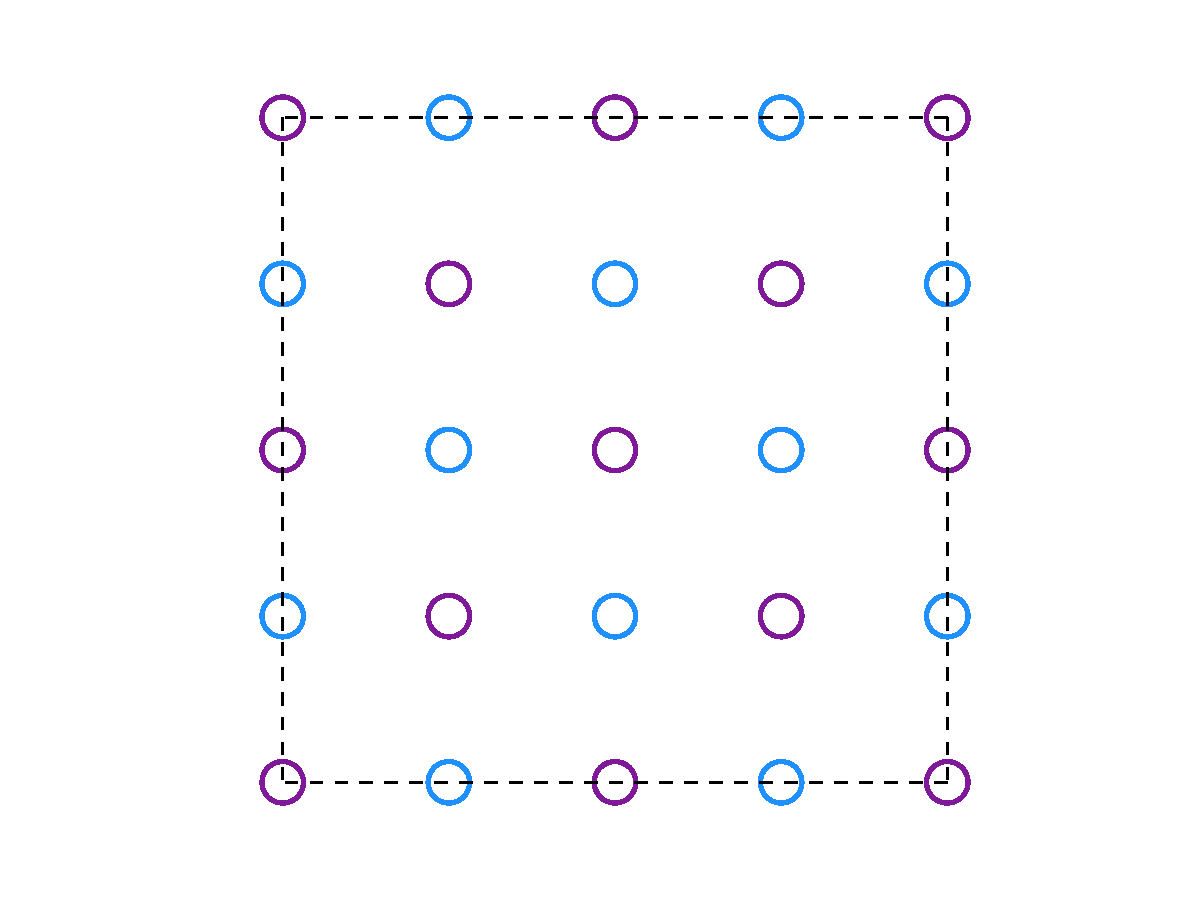
\includegraphics[width=0.5\textwidth]{layout.pdf}
%     \vspace{-15pt}
    \caption{The grid wind farm optimized in this study. When there were two groups, they were staggered in a checkerboard patter as shown.}
  \label{layout}
  \end{centering}
\end{figure}

% \vspace{-15pt}

In the second row of Fig \ref{unidirectional}, the optimal hub heights of each group are shown. There is a large height difference between the two groups for every case, with this optimal height difference decreasing slightly as the grid spacing increases. The large difference in height means that downstream wind turbines are partially out of the wake of upstream turbines from the large vertical distance between rotors. When the turbines are spaced farther apart, as in the 5.93 diameter grid, the losses cause by wakes are not as extreme, meaning that the power increase from decreased wake interference is not worth the increased cost of the much taller towers.
A similar trend is seen in the the bottom row in the optimal rotor diameters. In each case there is a large difference between the optimal rotor diameters of each group, with this difference decreasing for with increased grid spacing and shear exponent.

Because the wind direction is aligned with the rows in the grid, for the unidirectional wind rose there is a large benefit to using turbines with different heights and rotor diameters. The non-homogeneous turbines greatly decrease the wake interactions in the farm, resulting in a much lower COE. 



% \begin{figure}[htbp]
% \begin{centering}

% 	\subfloat[One wind direction.]{\includegraphics[width=0.499\textwidth]{rose1.pdf}\label{rose1}}
%     \subfloat[Two wind directions.]{\includegraphics[width=0.499\textwidth]{rose2.pdf}\label{rose2}}\\
%     \vspace{-0.5cm}
%     \subfloat[Three wind directions.]{\includegraphics[width=0.499\textwidth]{rose3.pdf}\label{rose3}}
%     \subfloat[Five wind directions.]{\includegraphics[width=0.499\textwidth]{rose4.pdf}\label{rose4}}\\
%     \subfloat[Three wind directions.]{\includegraphics[width=0.499\textwidth]{rose5.pdf}\label{rose5}}
%     \subfloat[Five wind directions.]{\includegraphics[width=0.499\textwidth]{rose6.pdf}\label{rose6}}
    
%   \caption{The wind distributions used in the different wind farm optimizations.}
%   \label{wind_roses}
%   \end{centering}
% \end{figure}



\begin{figure}[htbp]
\begin{centering}
	\subfloat{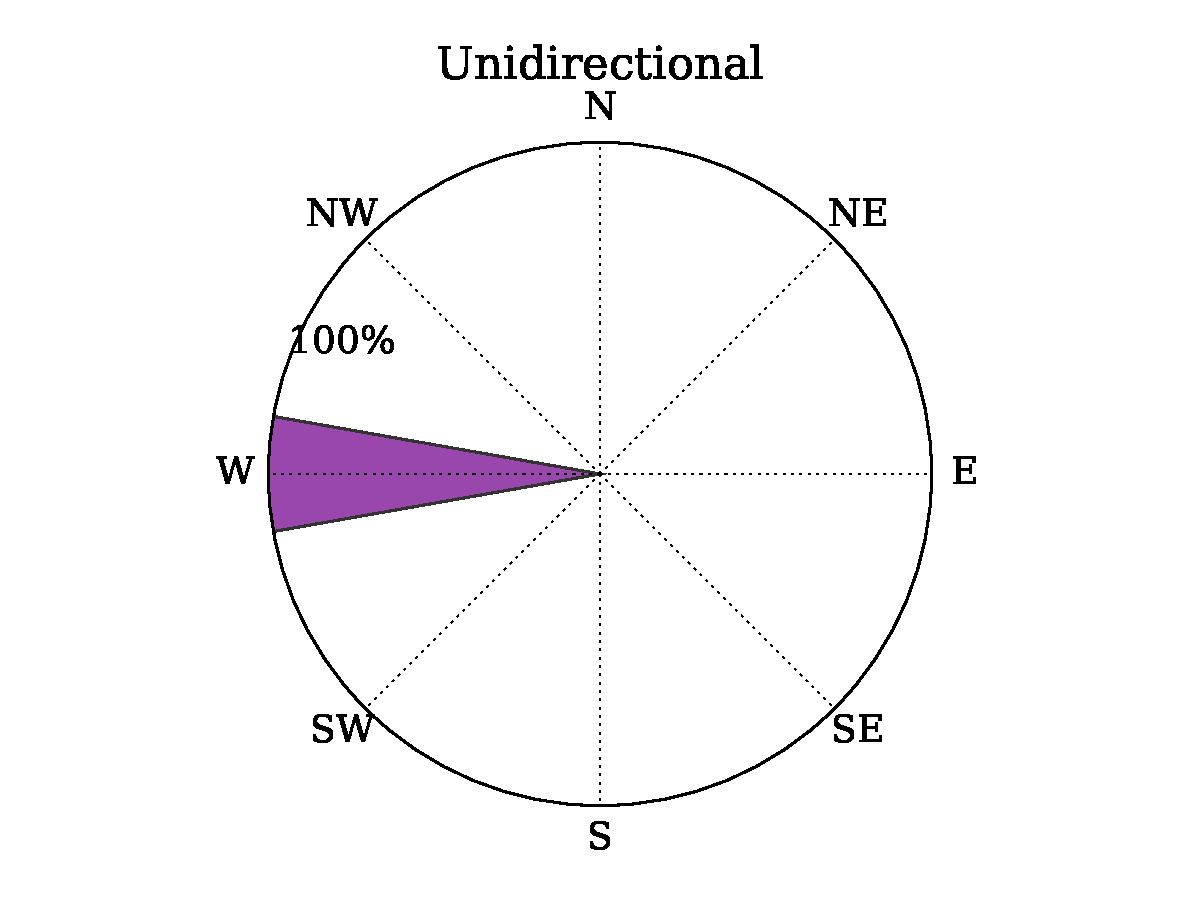
\includegraphics[width=0.35\textwidth]{unidirectional.pdf}} \\
    \vspace{-0.5cm}
	\subfloat{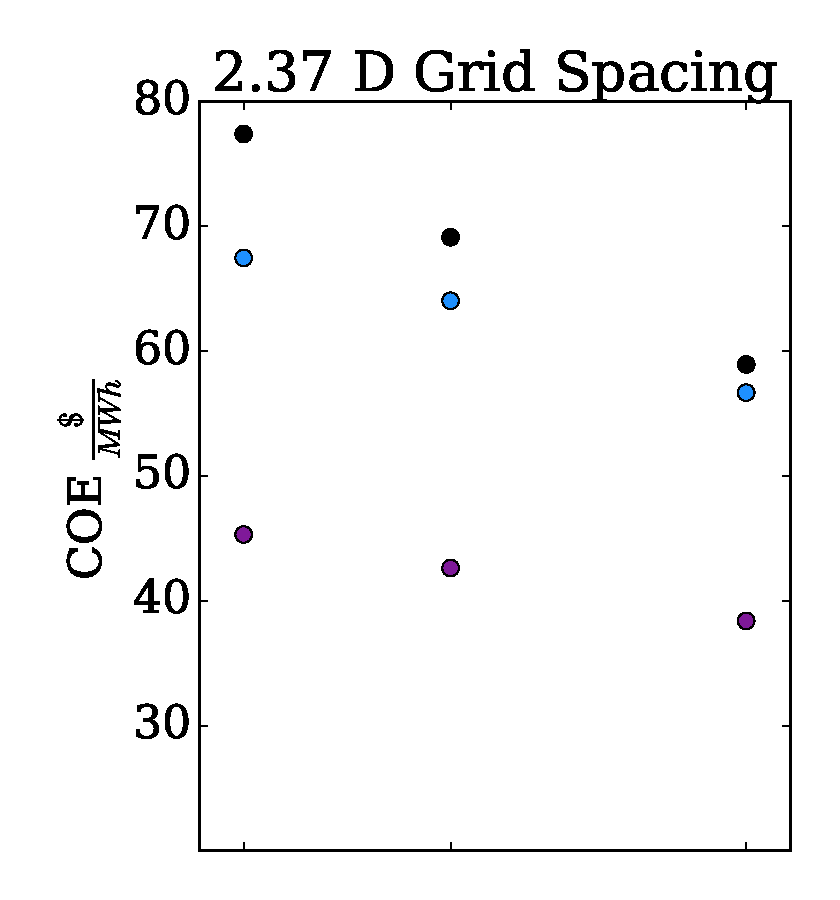
\includegraphics[height=0.305\textwidth]{1dir_300.pdf}}
    \hspace{-0.35cm}
    \subfloat{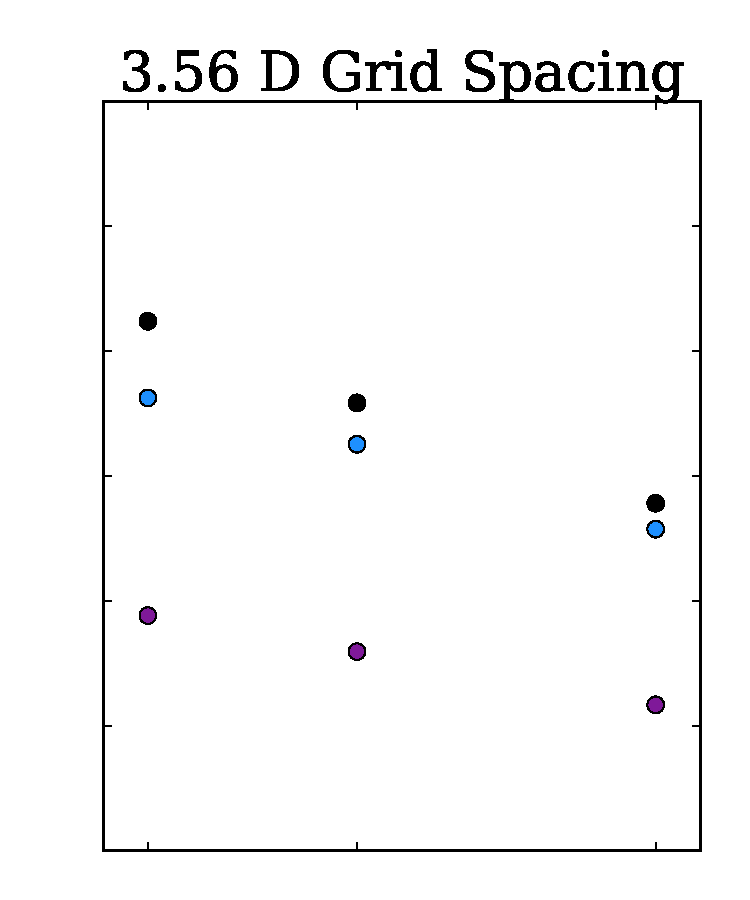
\includegraphics[height=0.305\textwidth]{1dir_450.pdf}}
    \hspace{-0.35cm}
    \subfloat{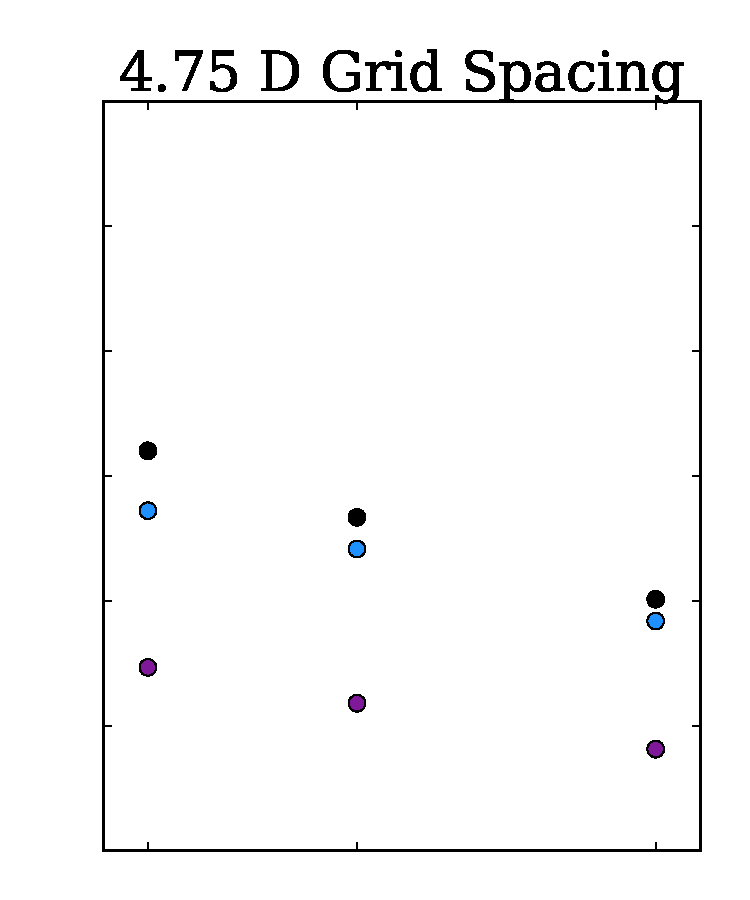
\includegraphics[height=0.305\textwidth]{1dir_600.pdf}}
    \hspace{-0.35cm}
    \subfloat{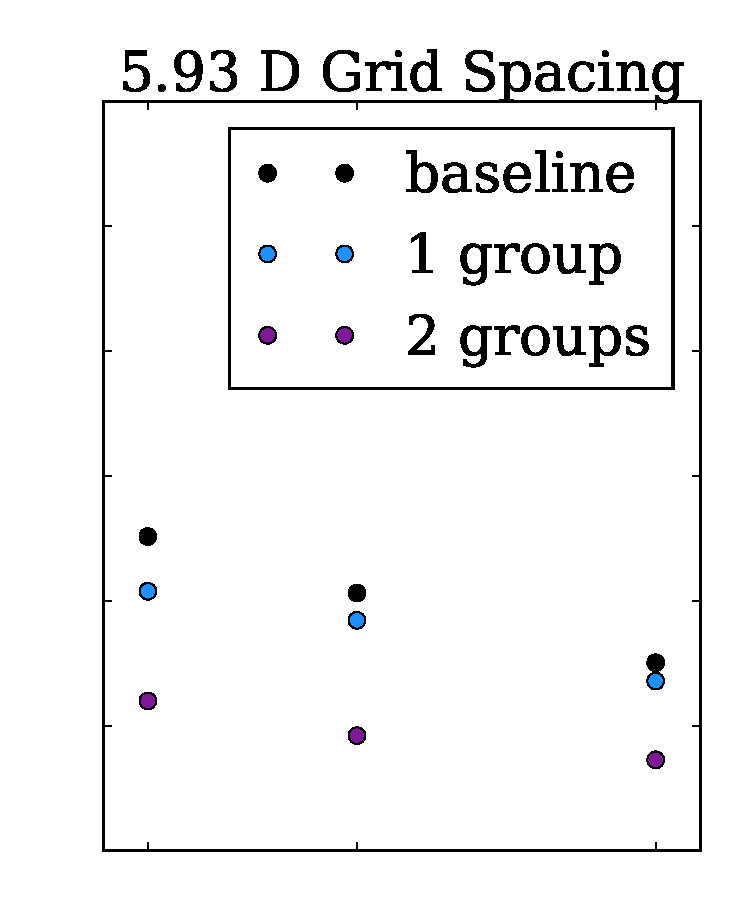
\includegraphics[height=0.305\textwidth]{1dir_750.pdf}}\\
%     \vspace{-0.7cm}
%     \subfloat{\includegraphics[width=0.15\textwidth]{legend.png}}\\
	\subfloat{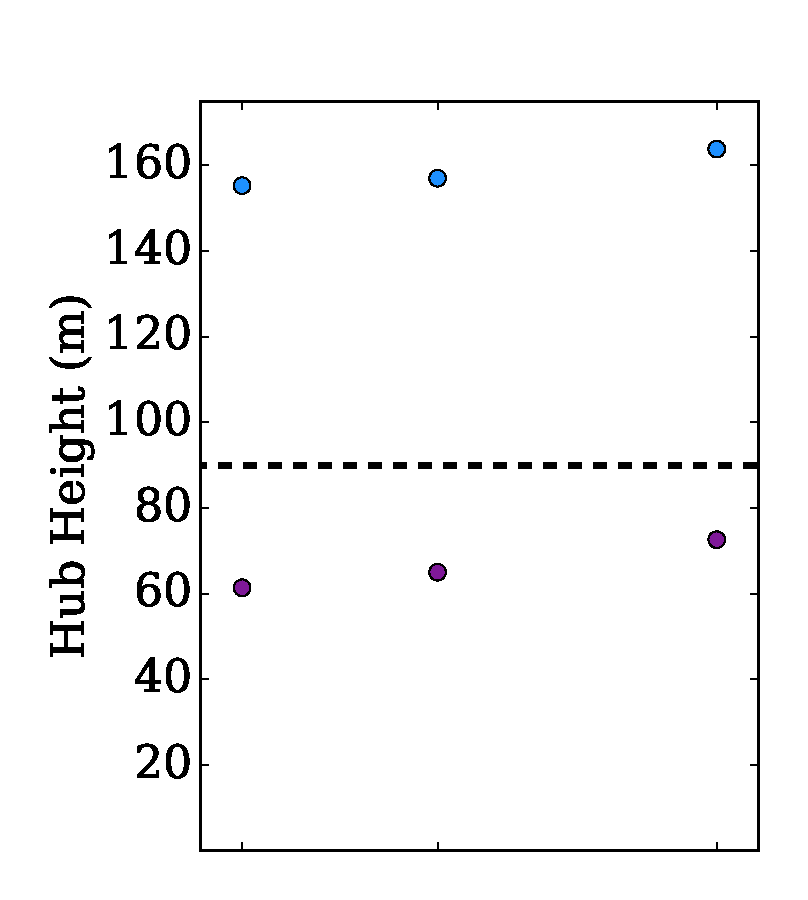
\includegraphics[height=0.305\textwidth]{H_1dir_300.pdf}}
    \hspace{-0.35cm}
    \subfloat{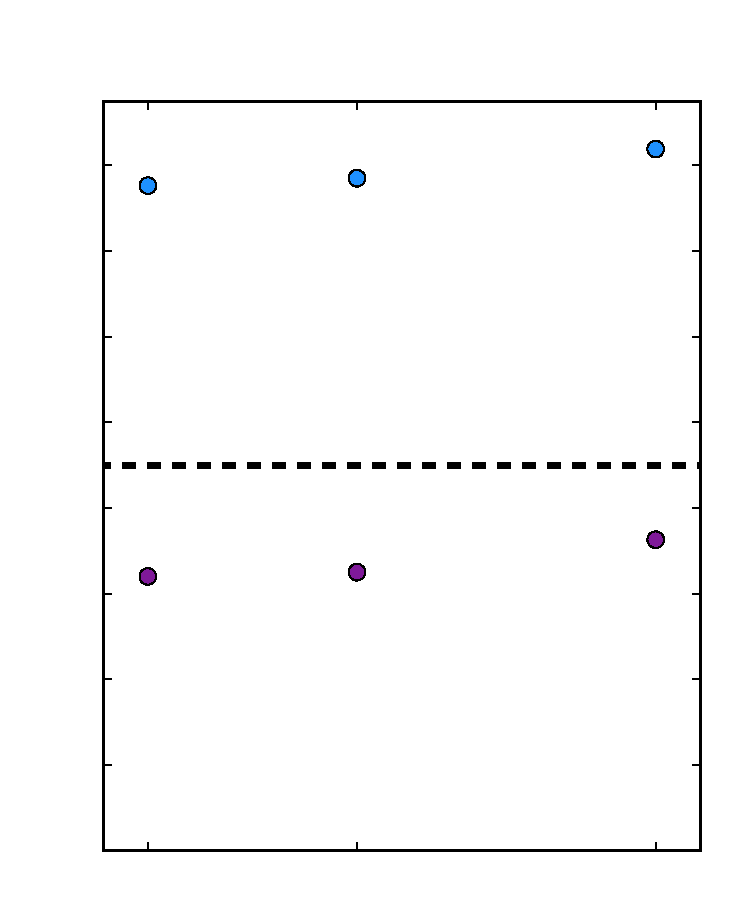
\includegraphics[height=0.305\textwidth]{H_1dir_450.pdf}}
    \hspace{-0.35cm}
    \subfloat{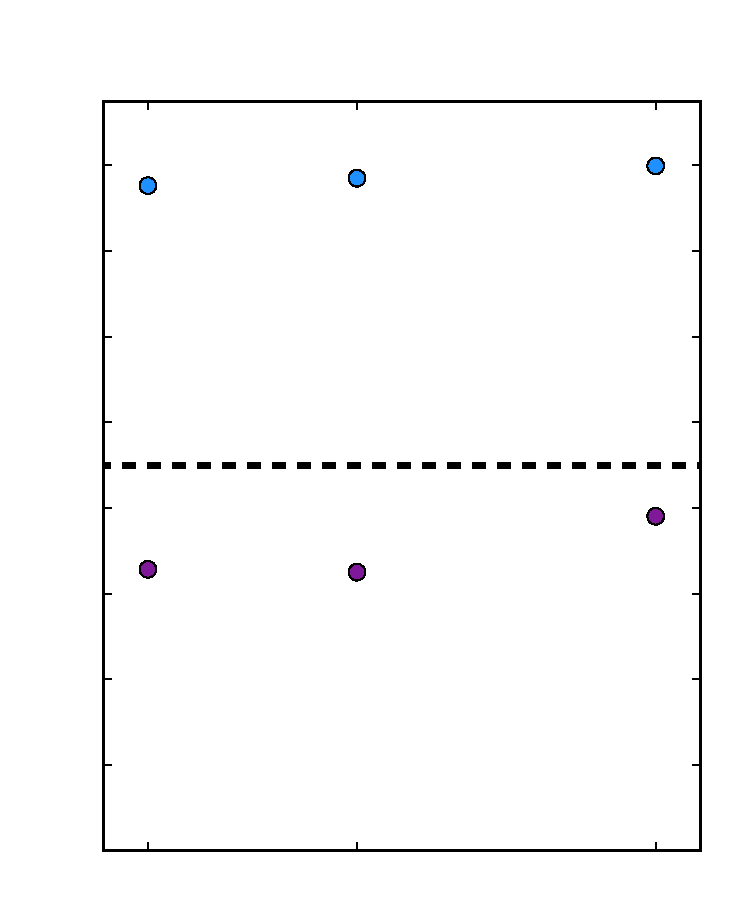
\includegraphics[height=0.305\textwidth]{H_1dir_600.pdf}}
    \hspace{-0.35cm}
    \subfloat{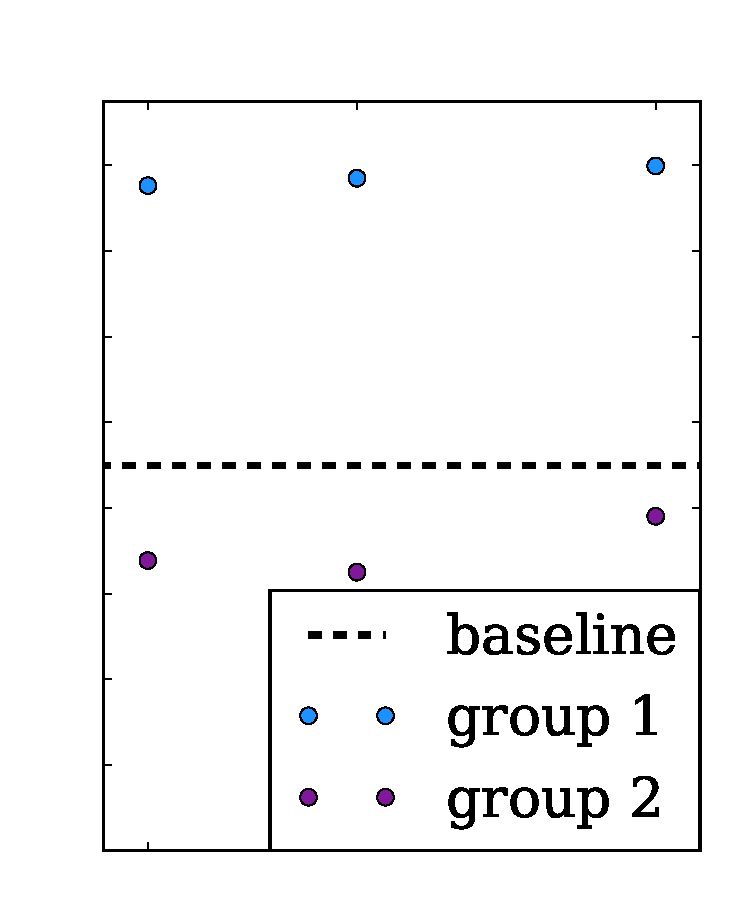
\includegraphics[height=0.305\textwidth]{H_1dir_750.pdf}}\\
%     \vspace{-0.7cm}
    \subfloat{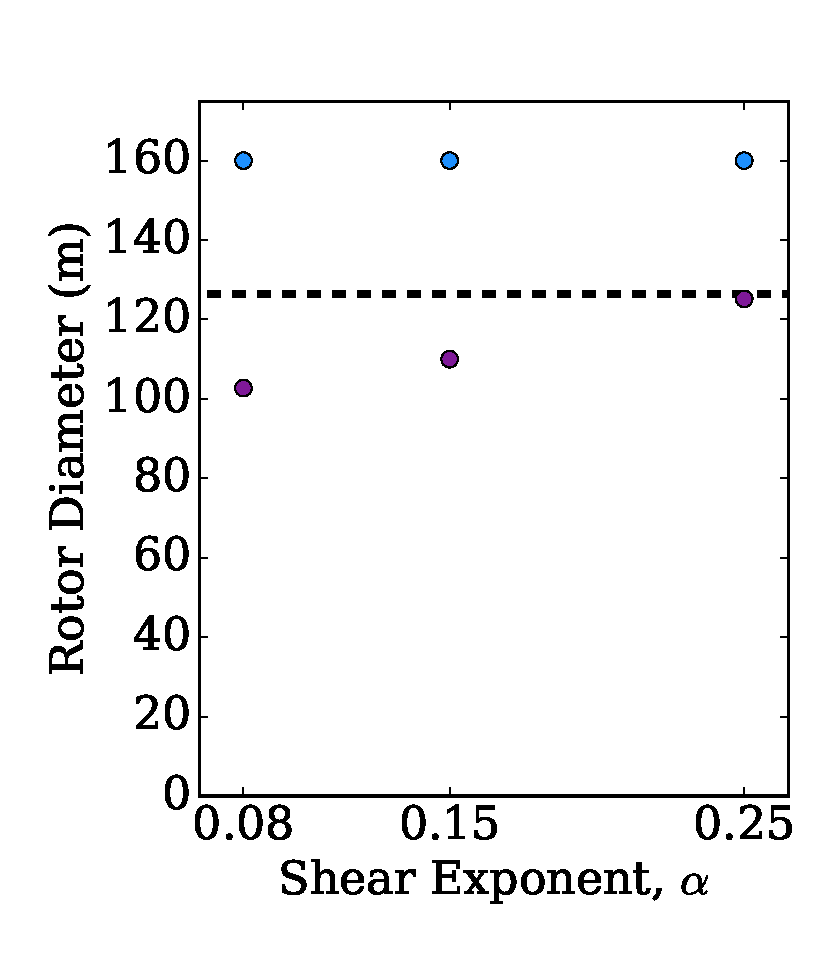
\includegraphics[width=0.2794\textwidth]{D_1dir_300.pdf}}
    \hspace{-0.35cm}
    \subfloat{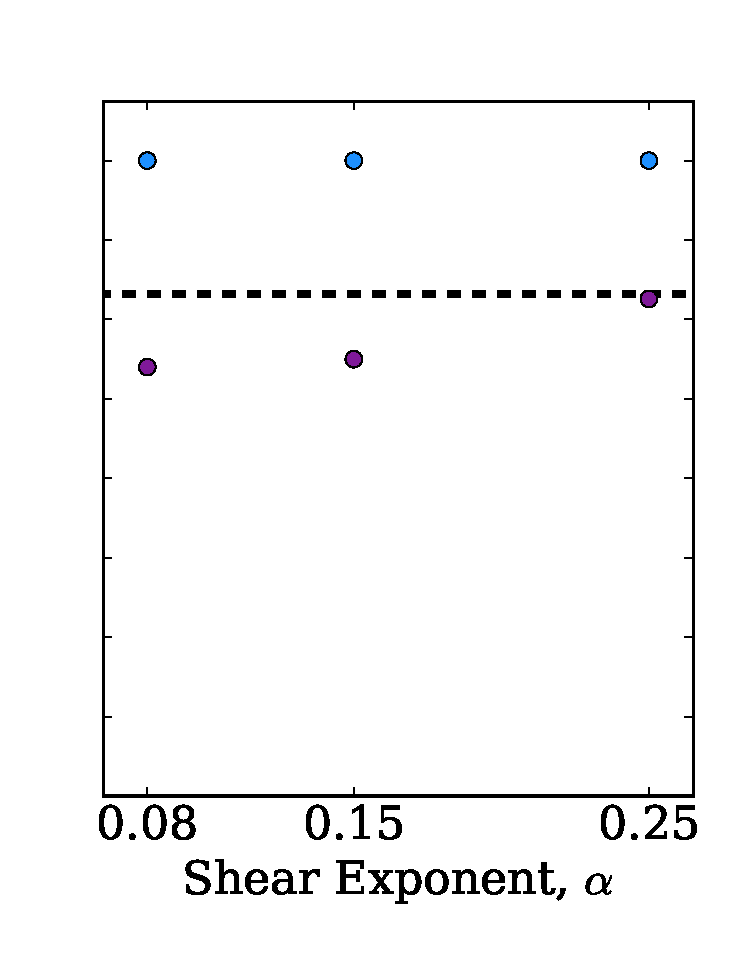
\includegraphics[width=0.25\textwidth]{D_1dir_450.pdf}}
    \hspace{-0.35cm}
    \subfloat{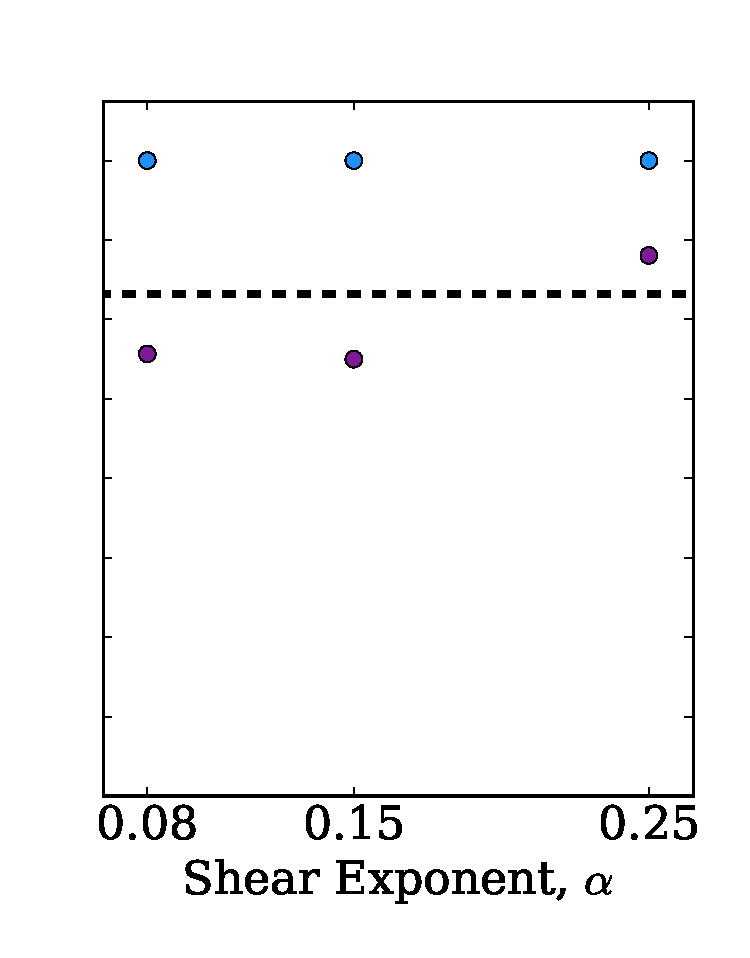
\includegraphics[width=0.25\textwidth]{D_1dir_600.pdf}}
    \hspace{-0.35cm}
    \subfloat{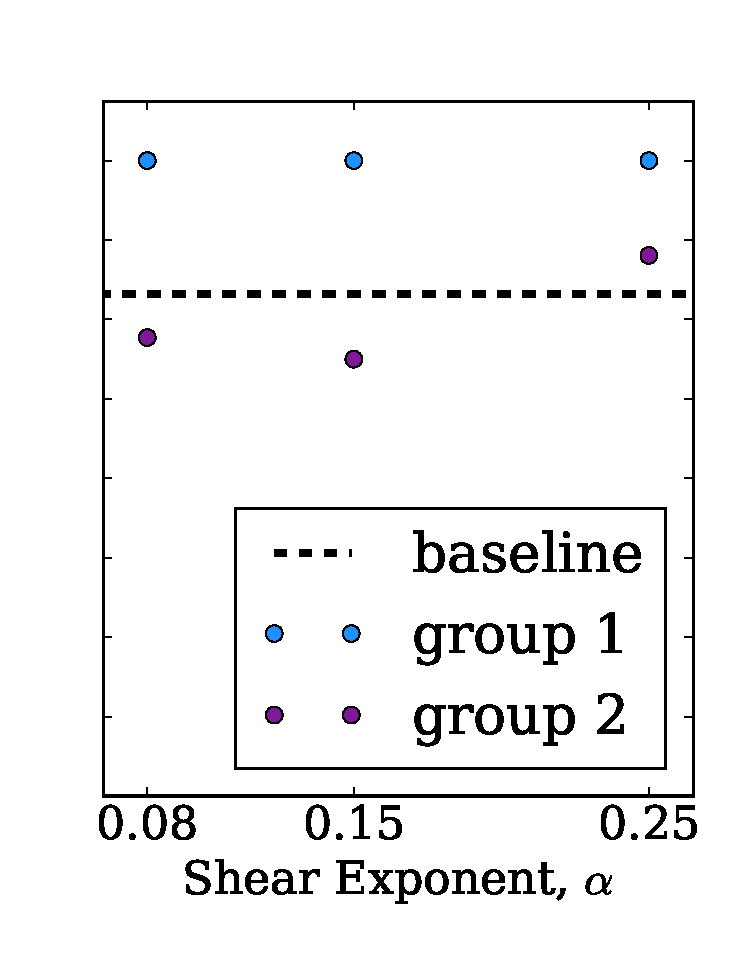
\includegraphics[width=0.25\textwidth]{D_1dir_750.pdf}}\\
    \vspace{-0.25cm}
    \caption{Optimization results for the unidirectional wind rose. The first row shows the COE, the second row shows optimal hub heights for each of the two groups, the third row shows optimal rotor diameters for each of the two groups. Each column represents a different grid spacing.}
  \label{unidirectional}
  \end{centering}
\end{figure}
    
%     \vspace{-7pt}
\subsection{West Dominant Wind Rose}
  Figure \ref{west} shows the results for the west dominant wind rose. Similar to the unidirectional case, the dominant wind direction for this wind rose is in line with the grid rows. For the 2.37 diameters grid spacing there is a large COE decrease between the farm with one turbine group to two. For a shear exponent of 0.08, turbines optimized uniformly decrease the COE by 10.2\% compared to the baseline, while two groups result in a COE decrease of 18.8\% compared to the baseline. At the 0.25 shear exponent, the COE decrease compared to baseline is 3.9\% and 11.3\% for one group and two groups, respectively.
  For the 3.56 diameter grid spacing, the COE decrease for one group compared to two is much smaller than the 2.37 diameter spacing, but still appreciable. With one height group, the COE decrease compared to the baseline is 11.2\%, 5.9\%, and 3.6\% for each of the shear exponents, while the COE decrease with two groups is 14.4\%, 11.5\% and 6.5\%.
For the 4.75 and 5.93 diameter grids, the COE for one turbine group and two turbine groups are similar or equal, with the exception of the 0.15 shear exponent and 4.75 diameter spacing with has a 6.2\% COE decrease with one group and 8.9\% COE decrease with two.
% For the 600 and 750 meter grid spacing, any benefit from two different groups is negligible, with perhaps the exception of the 600 meter grid spacing with a shear exponent of 0.15, which has a COE decrease of 4\% from one group to two. 
  
  The optimal hub heights and rotor diameters of the two groups are shown in the second an third rows of Fig. \ref{west}. For each grid spacings between 2.37 and 3.56 diameters and each shear exponent, there is a large height difference, around 70-80 meters, between the two groups.  The largest grid spacing has a much smaller height difference between the two groups, between 30 and 60 meters.
  The optimized rotor diameters for the lower two grid spacings trend towards large diameter differences for the lower shear exponents, and a smaller diameter difference for the larger shears. The 4.75 diameter grid spacing has fairly constant rotor diameter across the shear exponents. For the largest grid spacing the trend is reversed, the larger shear exponents have the greater difference in rotor diameter.
  
   Several optimization cases result in large differences between the turbine heights and rotor diameters of each group, but COE identical to that with just one turbine group. For the grid spacing of 4.75 and 5.93 diameters and shear values of 0.08 and 0.25, one and two groups both have the same COE. This behavior shows the intense multi-modality of the wind turbine design and farm optimization problem. The same low COE can be achieved with two drastically different wind farms. In these cases, two groups is not better than one, but is another way to achieve the same result. This same behavior can be seen in Fig. \ref{northwest} for the northwest wind rose.
    
    
    
\begin{figure}[htbp]
\begin{centering}
    \subfloat{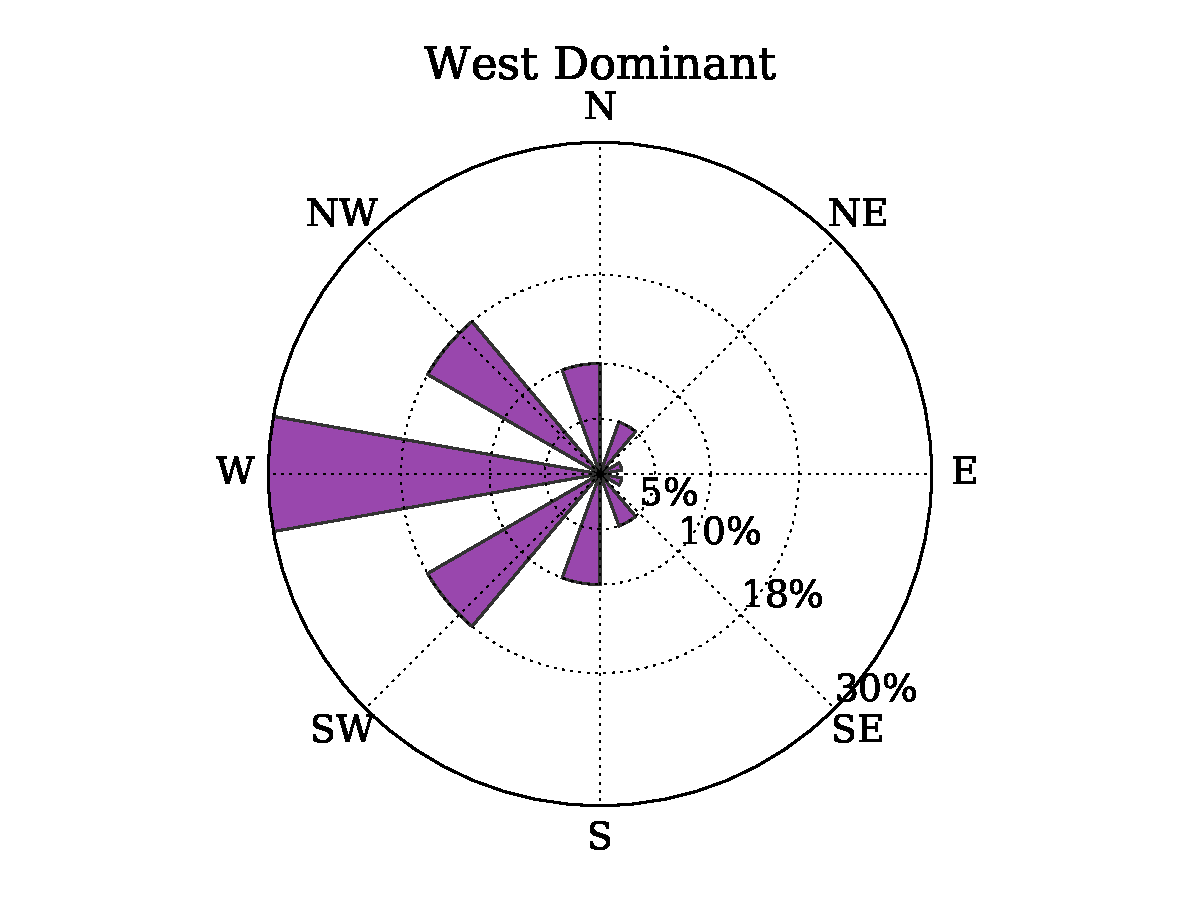
\includegraphics[width=0.35\textwidth]{west.pdf}} \\
    \vspace{-0.5cm}
	\subfloat{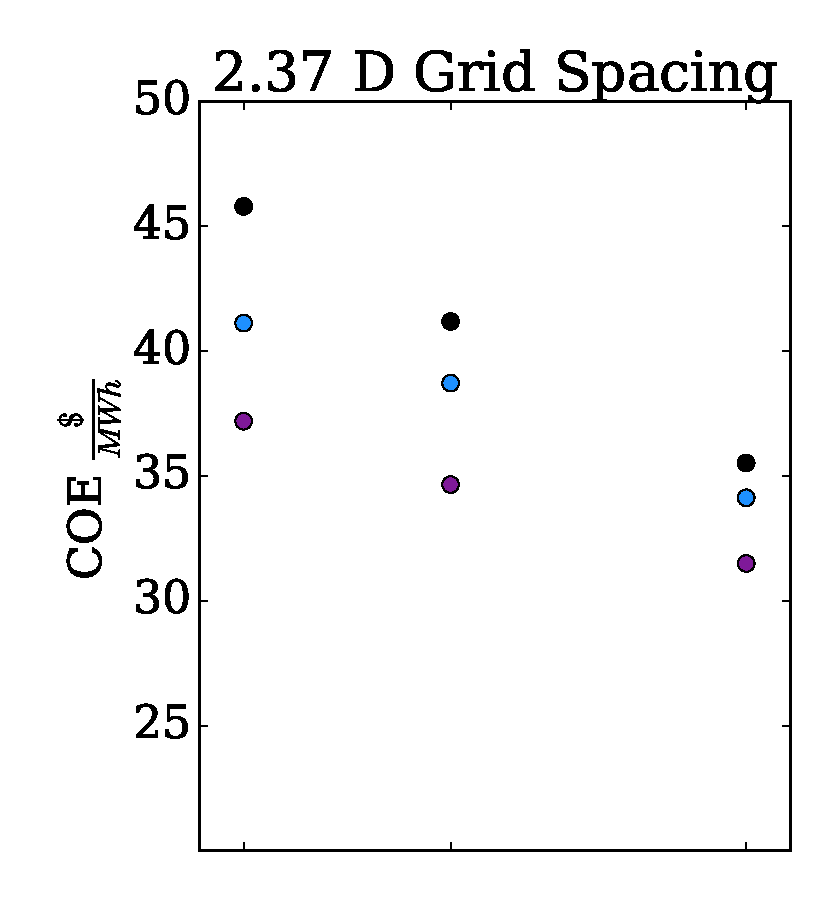
\includegraphics[height=0.305\textwidth]{W_300.pdf}}
    \hspace{-0.35cm}
    \subfloat{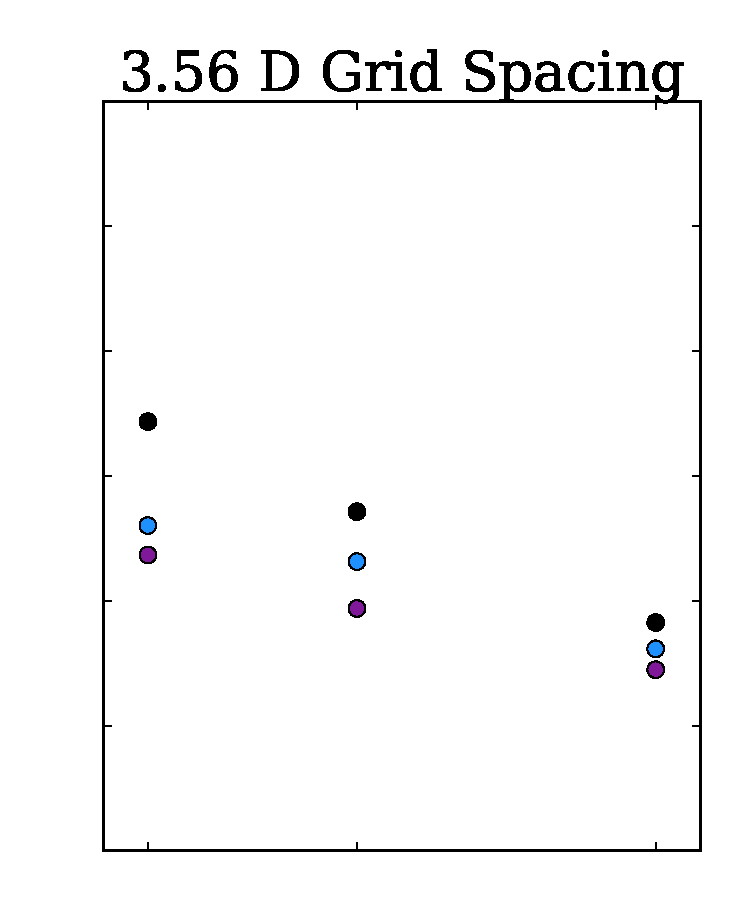
\includegraphics[height=0.305\textwidth]{W_450.pdf}}
    \hspace{-0.35cm}
    \subfloat{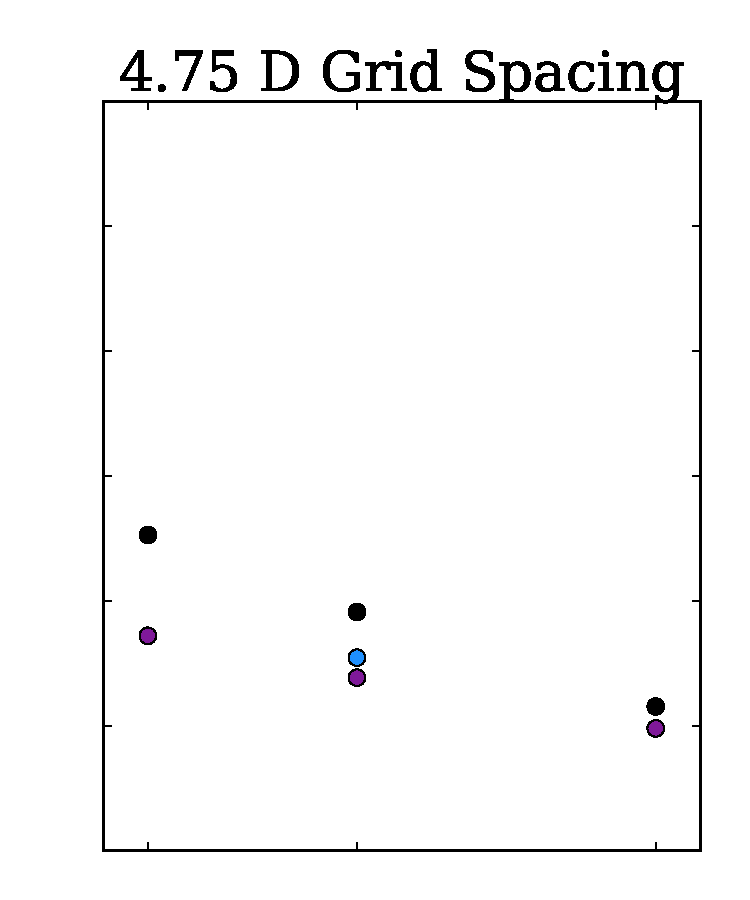
\includegraphics[height=0.305\textwidth]{W_600.pdf}}
    \hspace{-0.35cm}
    \subfloat{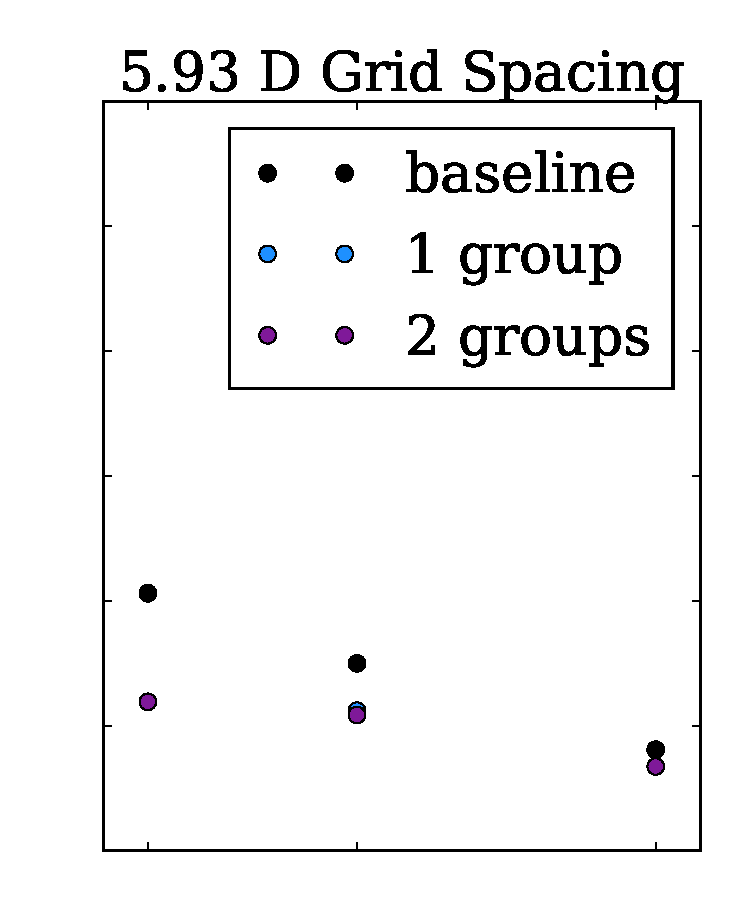
\includegraphics[height=0.305\textwidth]{W_750.pdf}}\\
%     \vspace{-0.7cm}
%     \subfloat{\includegraphics[width=0.15\textwidth]{legend.png}}\\
	\subfloat{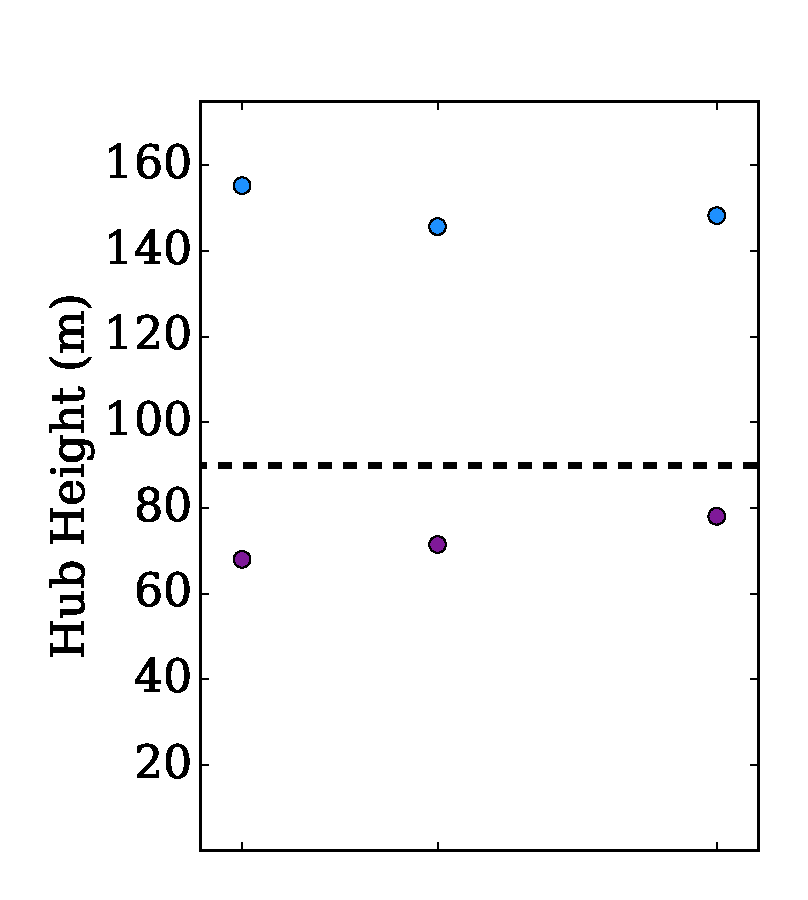
\includegraphics[height=0.305\textwidth]{H_W_300.pdf}}
    \hspace{-0.35cm}
    \subfloat{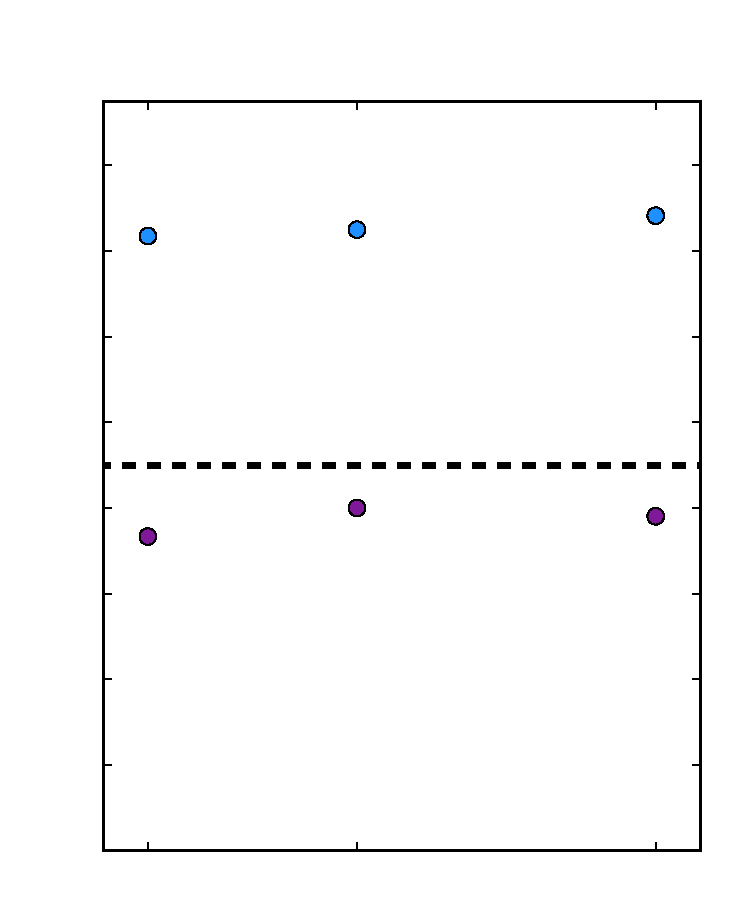
\includegraphics[height=0.305\textwidth]{H_W_450.pdf}}
    \hspace{-0.35cm}
    \subfloat{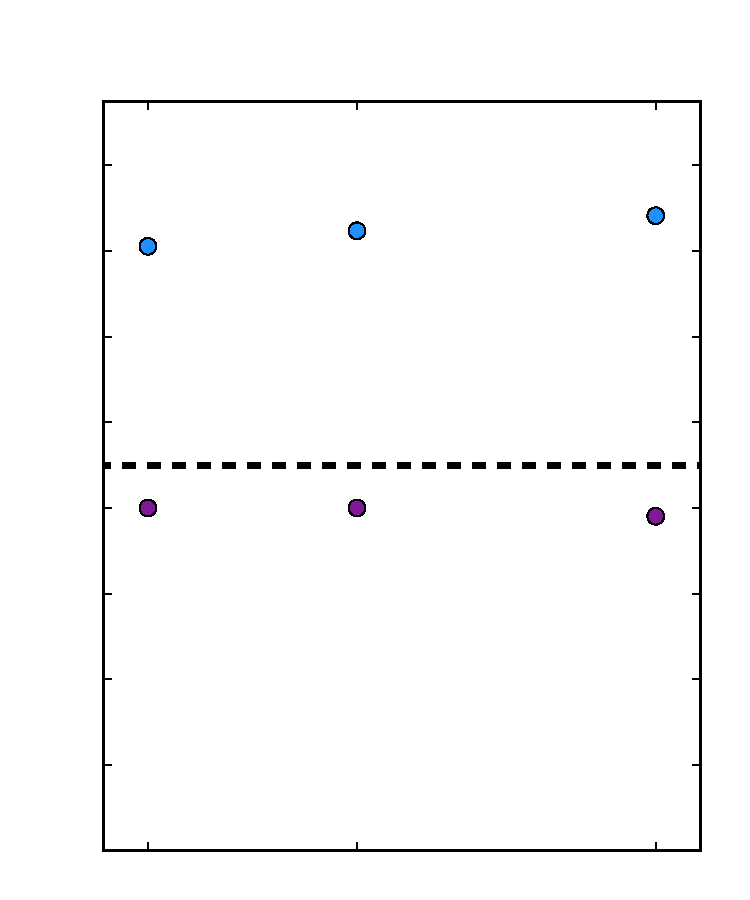
\includegraphics[height=0.305\textwidth]{H_W_600.pdf}}
    \hspace{-0.35cm}
    \subfloat{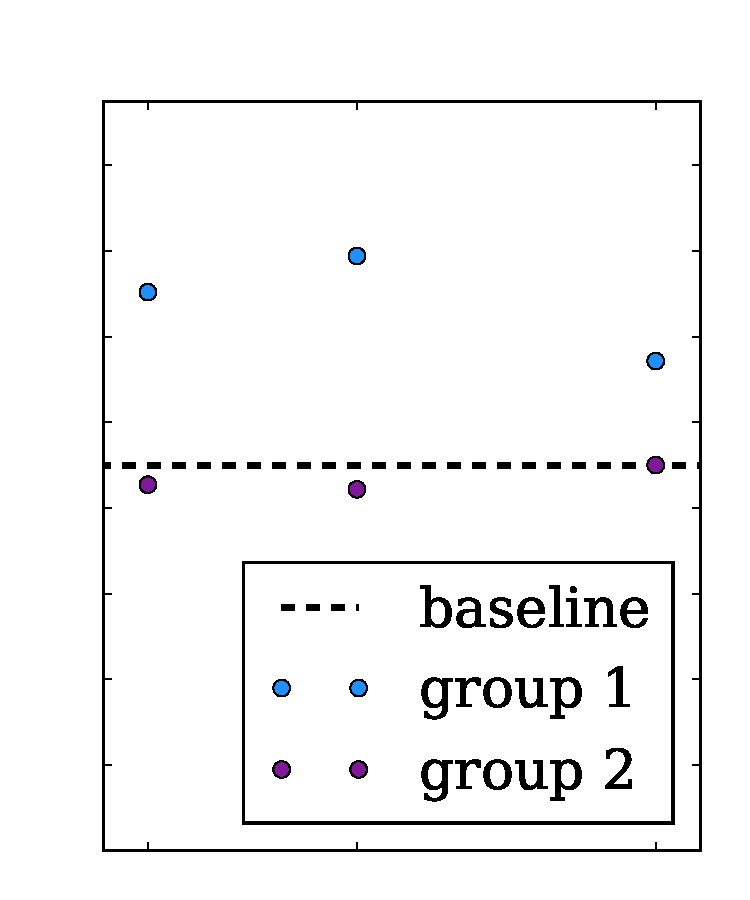
\includegraphics[height=0.305\textwidth]{H_W_750.pdf}}\\
%     \vspace{-0.7cm}
    \subfloat{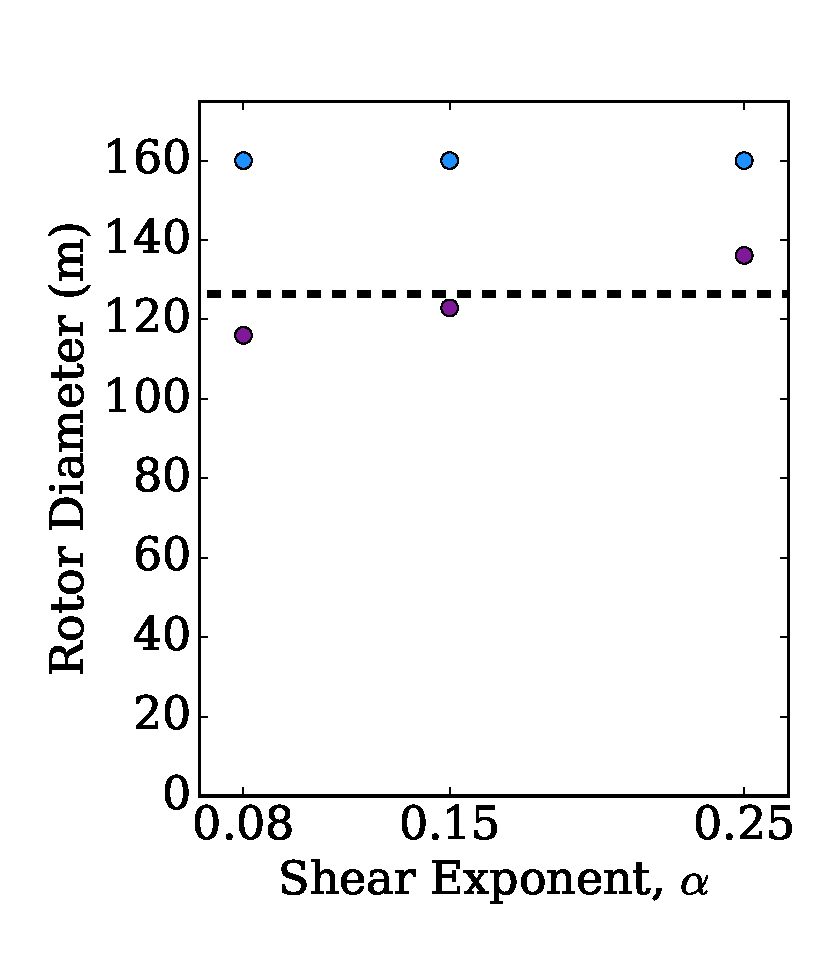
\includegraphics[width=0.2794\textwidth]{D_W_300.pdf}}
    \hspace{-0.35cm}
    \subfloat{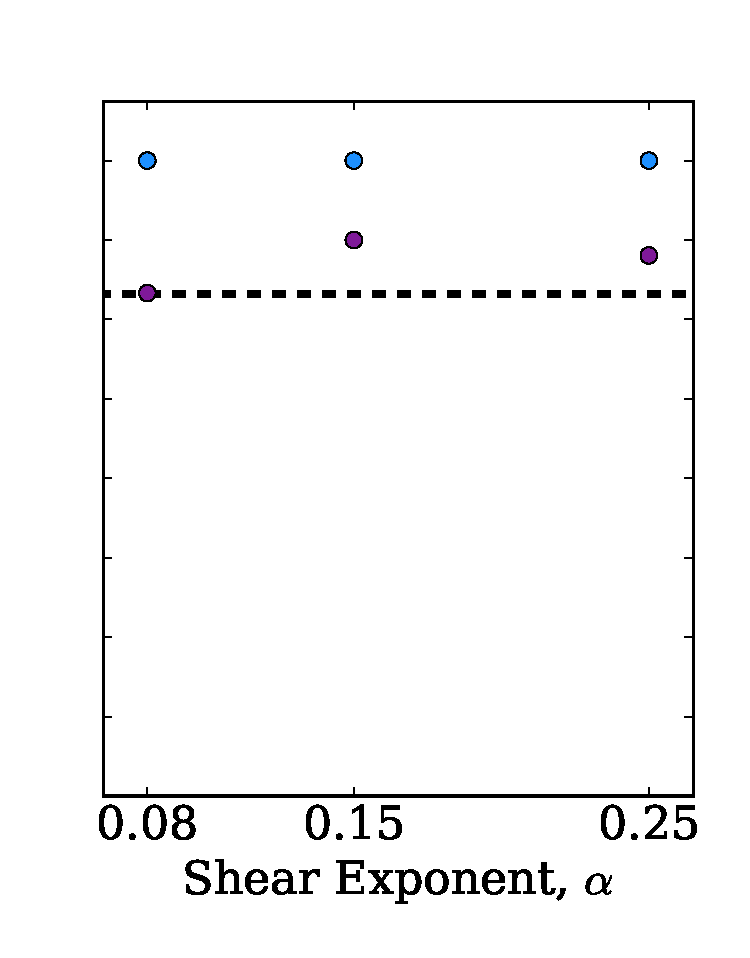
\includegraphics[width=0.25\textwidth]{D_W_450.pdf}}
    \hspace{-0.35cm}
    \subfloat{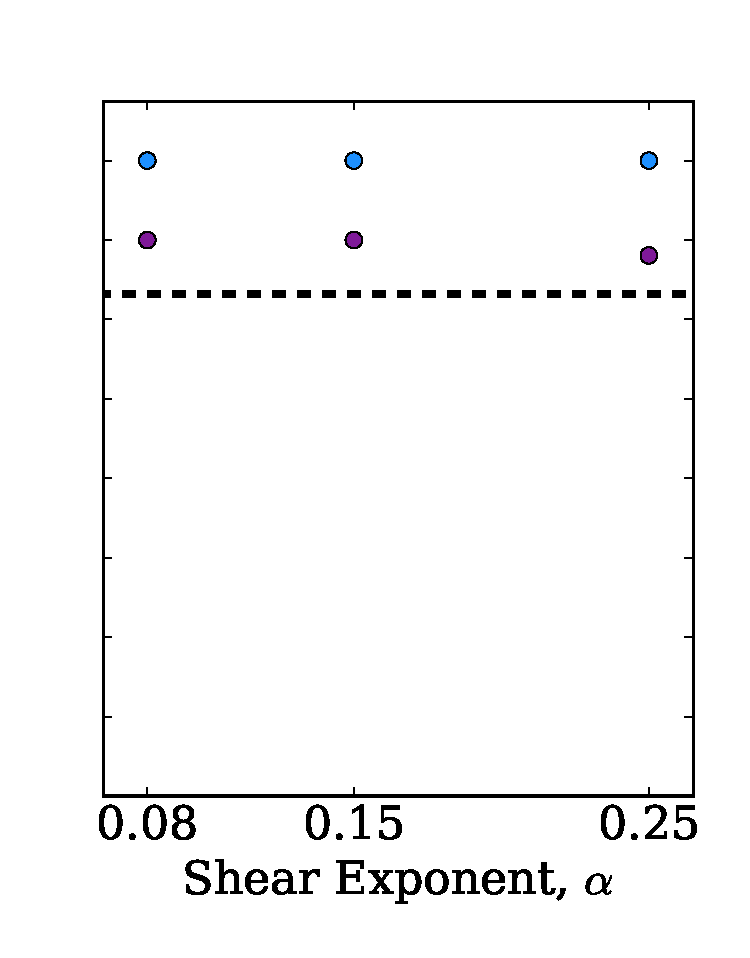
\includegraphics[width=0.25\textwidth]{D_W_600.pdf}}
    \hspace{-0.35cm}
    \subfloat{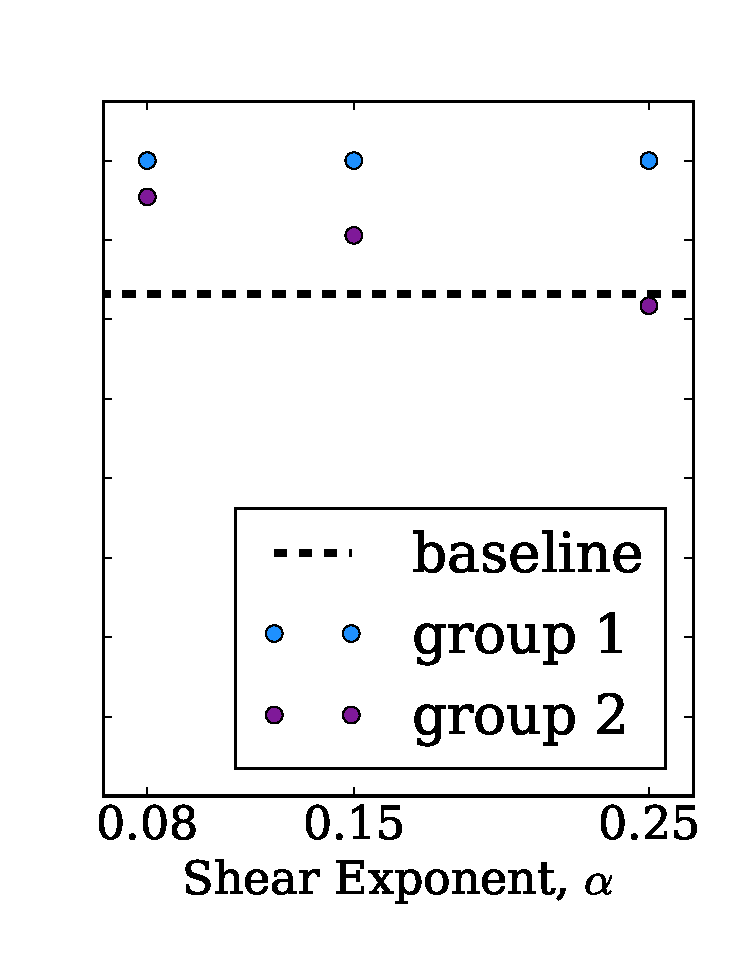
\includegraphics[width=0.25\textwidth]{D_W_750.pdf}}\\
    \vspace{-0.25cm}
    \caption{Optimization results for the west dominant wind rose. The first row shows the COE, the second row shows optimal hub heights for each of the two groups, the third row shows optimal rotor diameters for each of the two groups. Each column represents a different grid spacing.}
  \label{west}
  \end{centering}
\end{figure}
   
%    \vspace{-7pt}
   \subsection{Northwest Wind Rose}
   Figure \ref{northwest} displays the optimization results for the northwest dominant wind rose. The optimal COE results are very similar to Fig. \ref{west}. 
   Compared to the baseline, the 2.37 diameter grid wind farm has a COE decrease of 9.8\%, 5.8\%, and 4.0\% for each of the wind shear exponents and one turbine design group. For two groups, the COE decrease is 16.6\%, 14.2\% and 10.5\% from the baseline. 
   The 3.56 diameter grid has optimal COE for two groups much more similar to that with just one group. From baseline, one optimal group decreases COE 11.3\%, 6.1\%, and 2.4\% for each of the shear exponents, while two groups decrease the COE 14.0\%, 10.6\%, and 4.7\%. Have two different groups is still beneficial in this case, however not nearly as beneficial as it was when the turbines were closer together. 
   For the larger grid spacings, the COE decrease from baseline is practically the same for one turbine group compared to two. At most, two turbine groups gives an additional COE decrease of less than 3\%. 
%    The largest COE decrease between one and two groups occurs at the 300 meter grid spacing, varying from 7\% to 9\%. For the 450 meter grid spacing, this COE decrease between one and two groups ranges from 1\% to 5\%. There is minimal COE decrease between one and two groups for the 600 and 750 meter grid spacing.
   The turbine hub heights and rotor diameters for this wind rose follow a similar trend to that in Fig. \ref{west} for the west wind rose. 
  
   
%    the large rotor diameter difference only demonstrates the multi-modality of this function space, not the benefit to different rotor diameters.
   
   
   
\begin{figure}[htbp]
\begin{centering}
    \subfloat{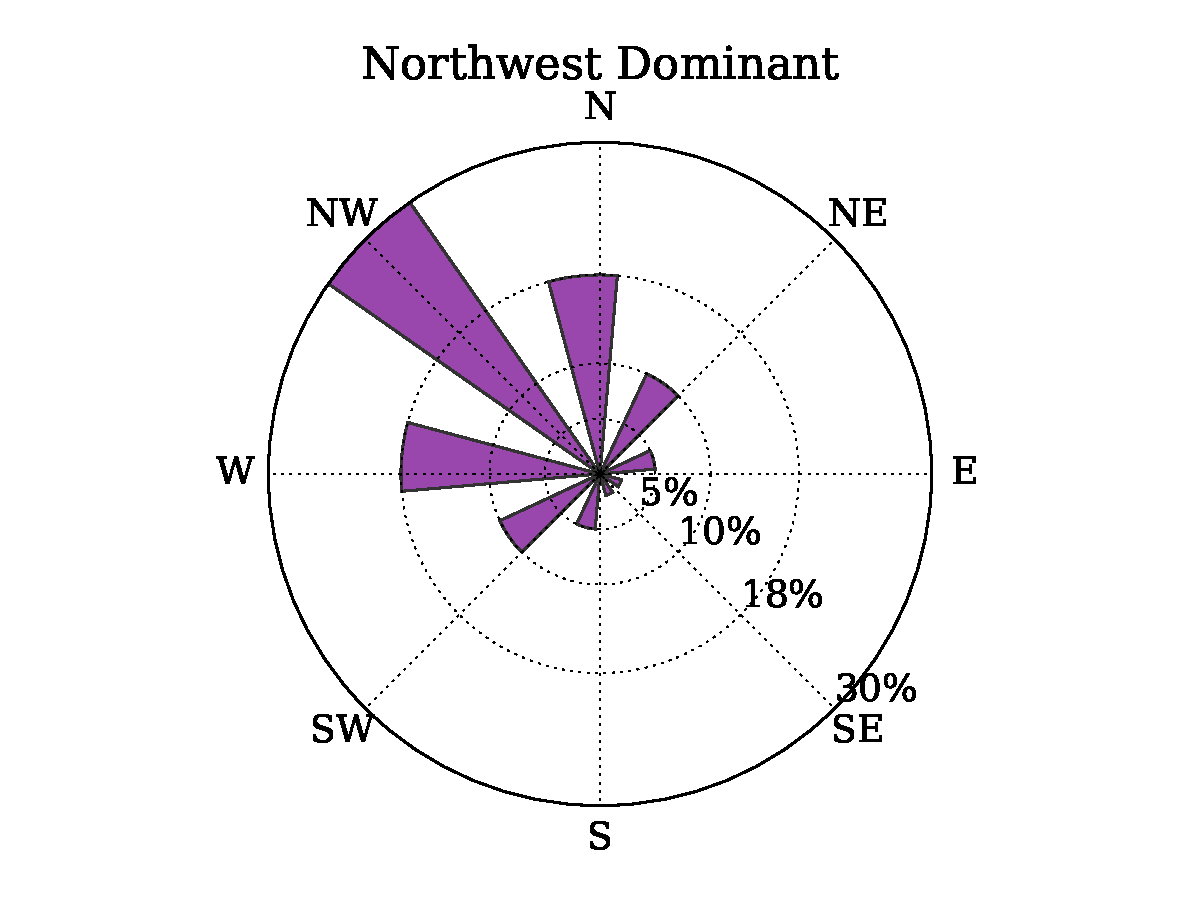
\includegraphics[width=0.35\textwidth]{northwest.pdf}} \\
    \vspace{-0.5cm}
	\subfloat{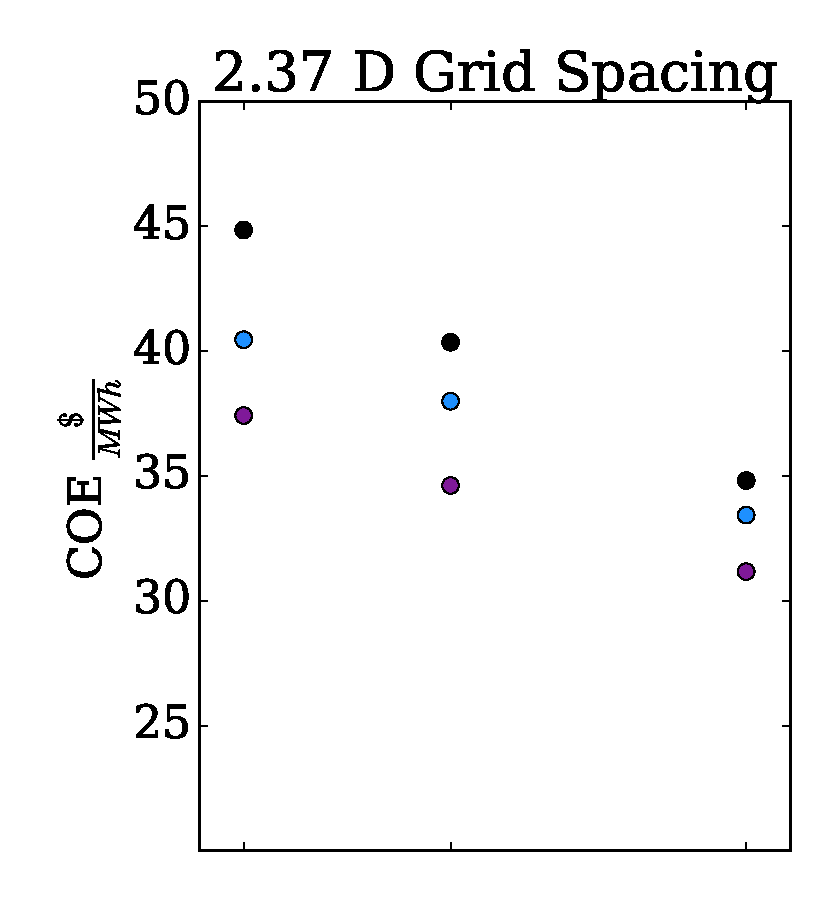
\includegraphics[height=0.305\textwidth]{NW_300.pdf}}
    \hspace{-0.35cm}
    \subfloat{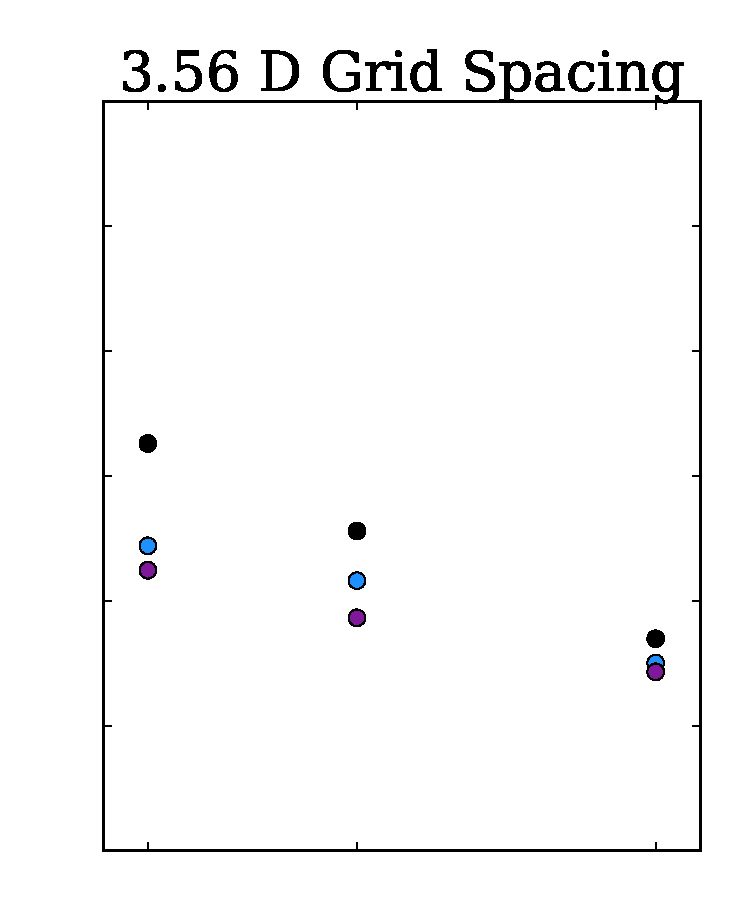
\includegraphics[height=0.305\textwidth]{NW_450.pdf}}
    \hspace{-0.35cm}
    \subfloat{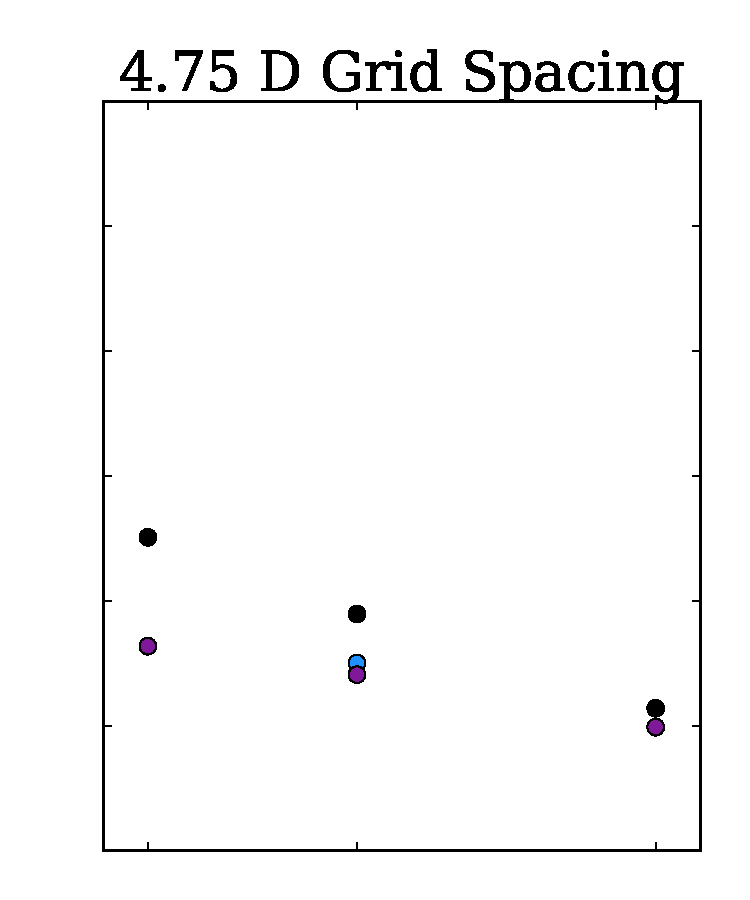
\includegraphics[height=0.305\textwidth]{NW_600.pdf}}
    \hspace{-0.35cm}
    \subfloat{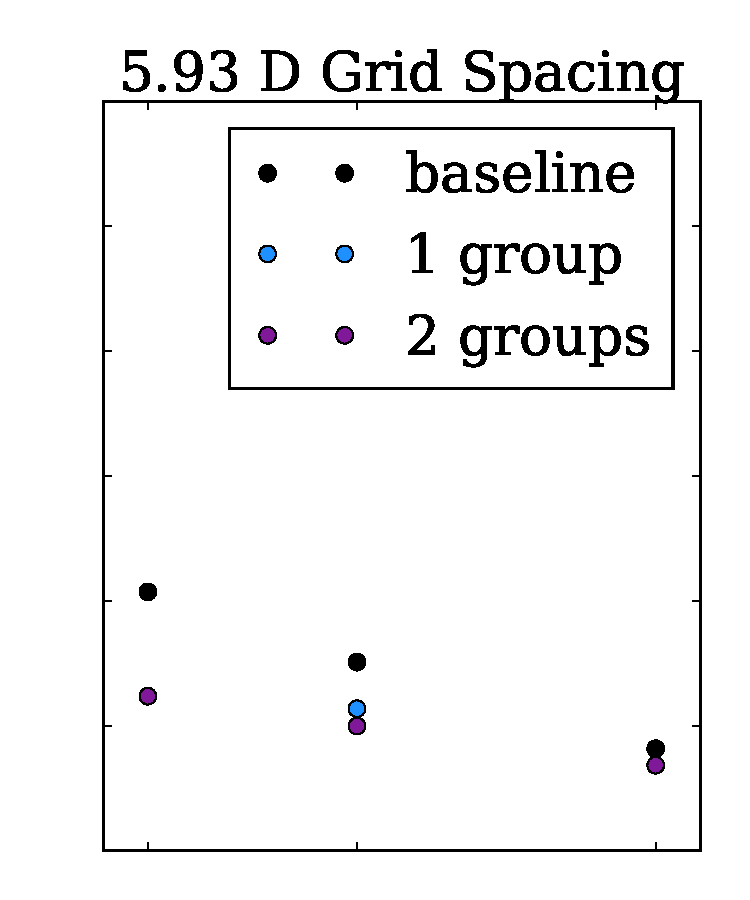
\includegraphics[height=0.305\textwidth]{NW_750.pdf}}\\
%     \vspace{-0.7cm}
%     \subfloat{\includegraphics[width=0.15\textwidth]{legend.png}}\\
	\subfloat{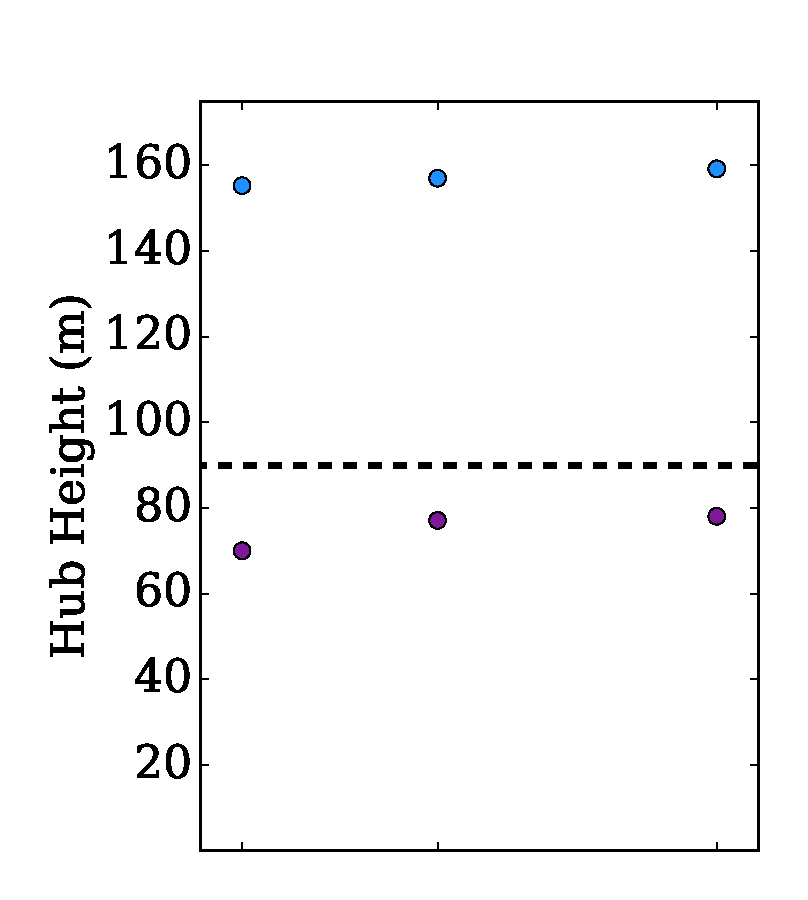
\includegraphics[height=0.305\textwidth]{H_NW_300.pdf}}
    \hspace{-0.35cm}
    \subfloat{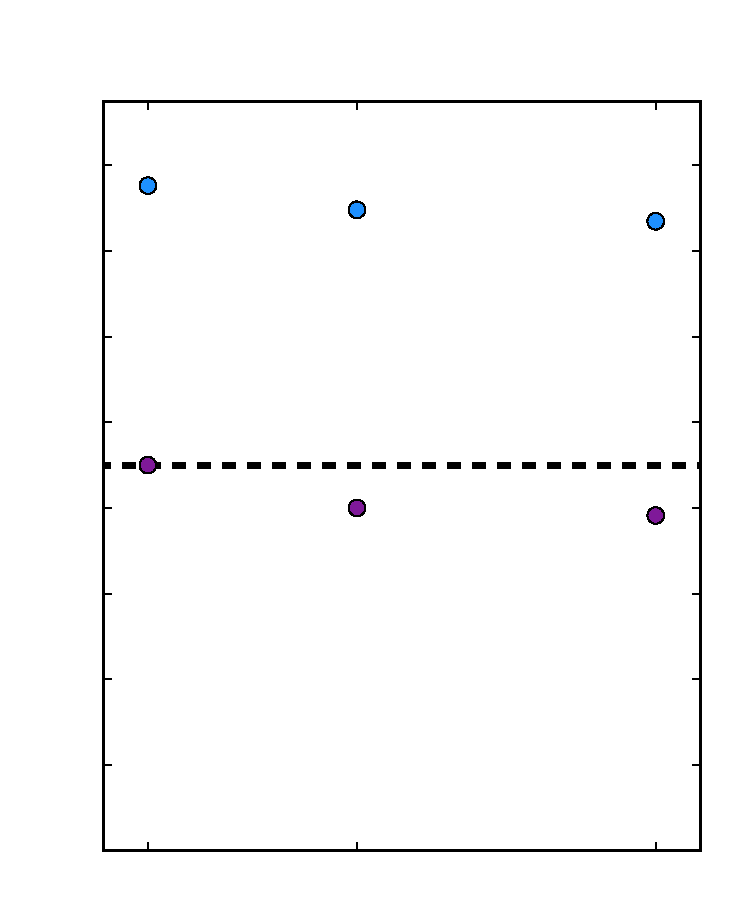
\includegraphics[height=0.305\textwidth]{H_NW_450.pdf}}
    \hspace{-0.35cm}
    \subfloat{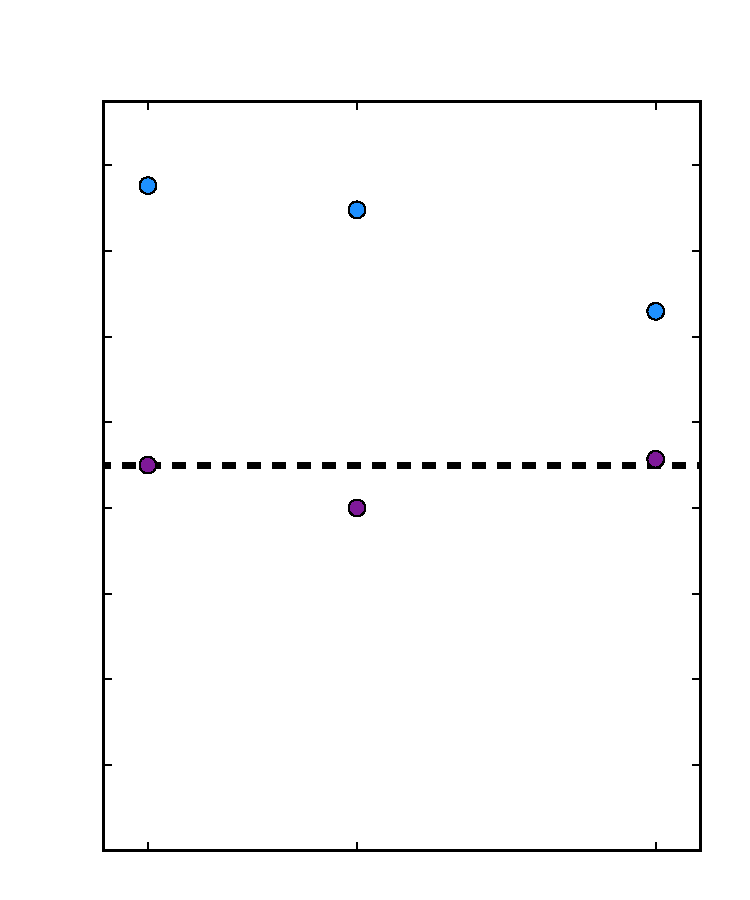
\includegraphics[height=0.305\textwidth]{H_NW_600.pdf}}
    \hspace{-0.35cm}
    \subfloat{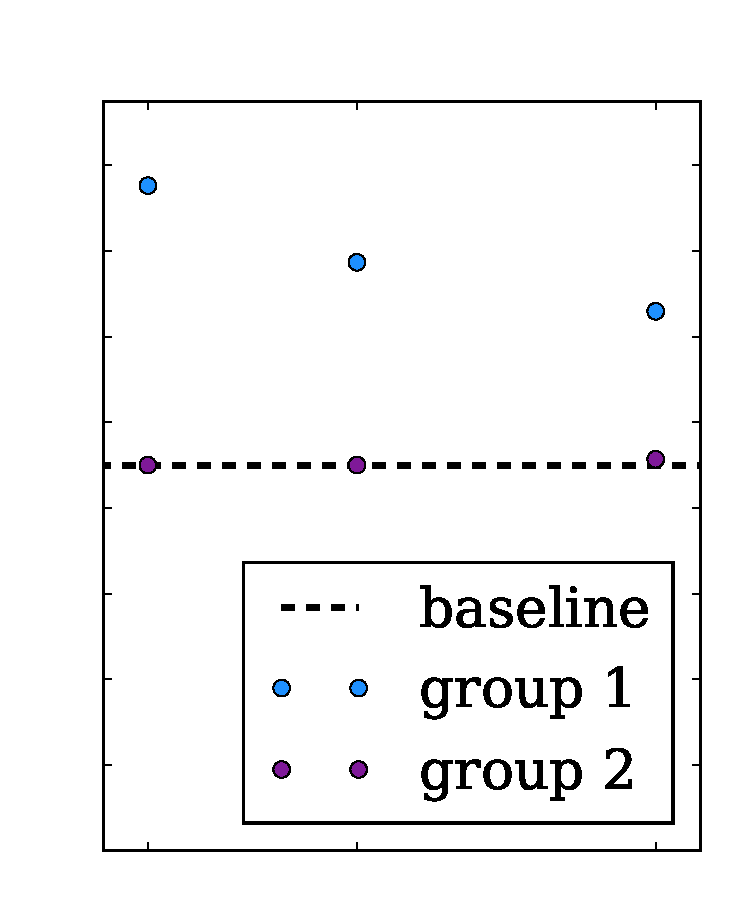
\includegraphics[height=0.305\textwidth]{H_NW_750.pdf}}\\
%     \vspace{-0.7cm}
    \subfloat{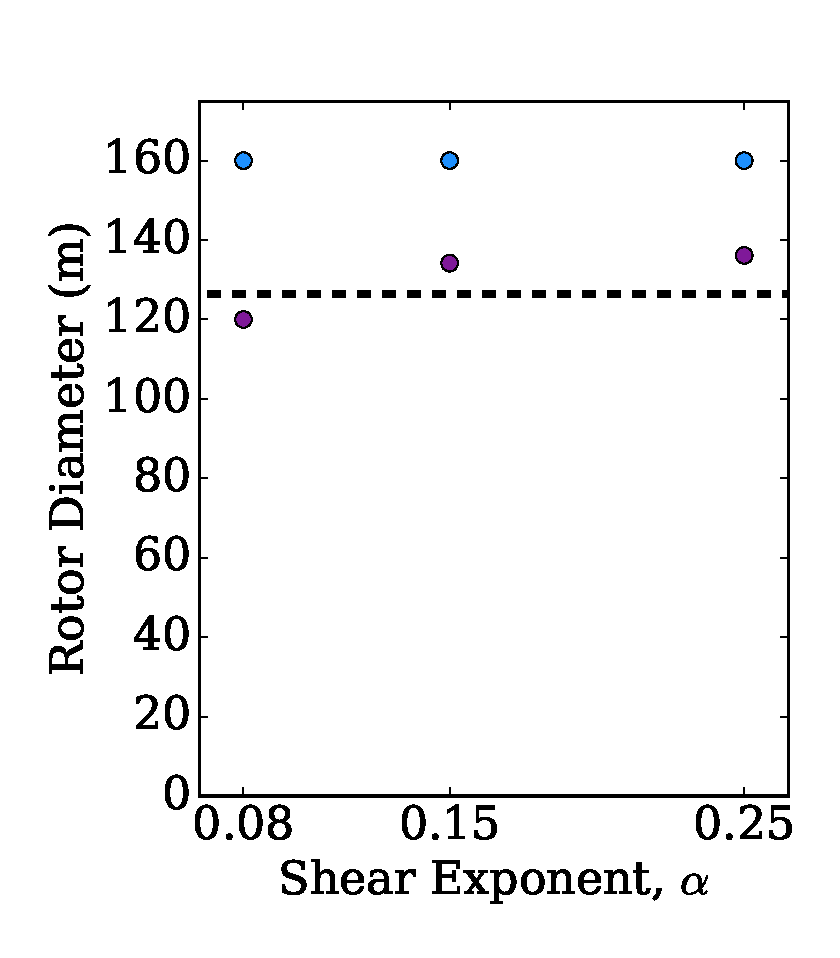
\includegraphics[width=0.2794\textwidth]{D_NW_300.pdf}}
    \hspace{-0.35cm}
    \subfloat{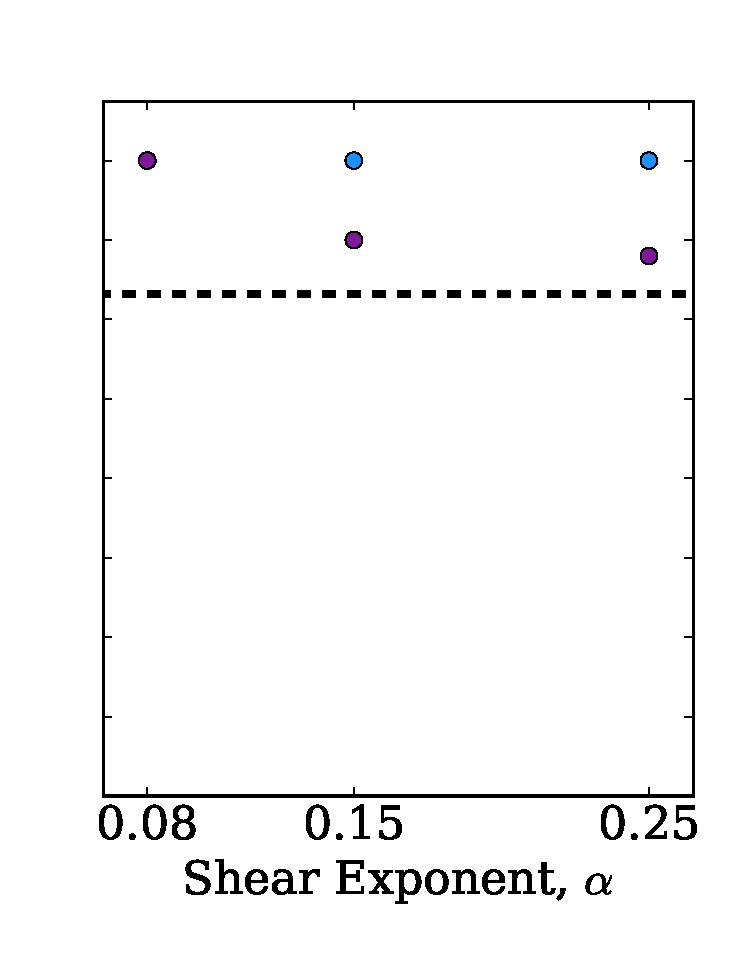
\includegraphics[width=0.25\textwidth]{D_NW_450.pdf}}
    \hspace{-0.35cm}
    \subfloat{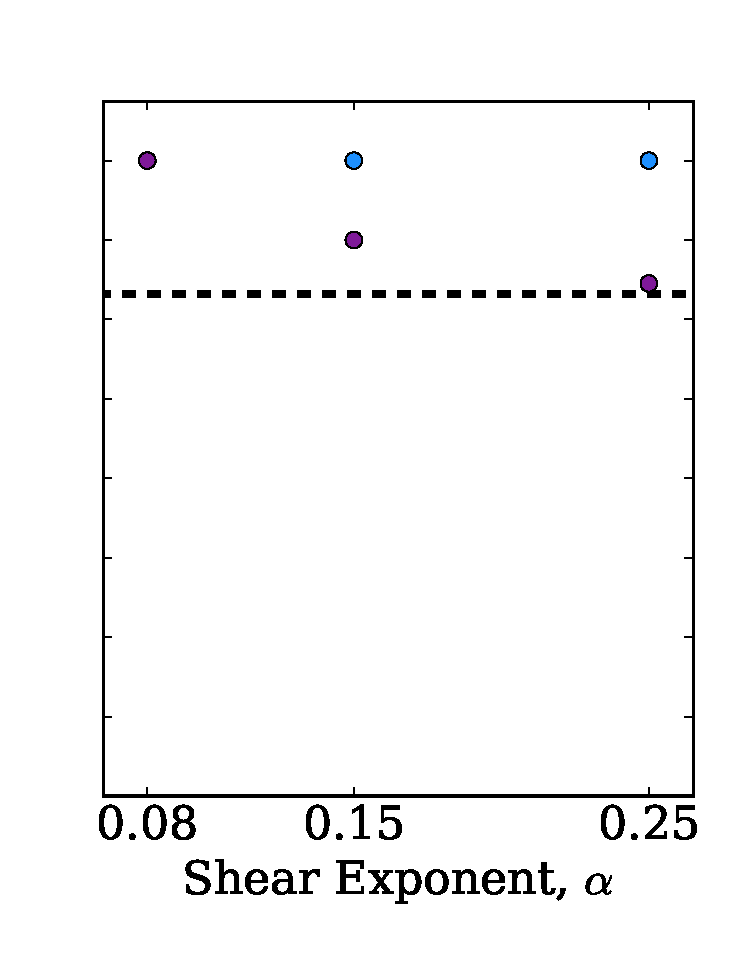
\includegraphics[width=0.25\textwidth]{D_NW_600.pdf}}
    \hspace{-0.35cm}
    \subfloat{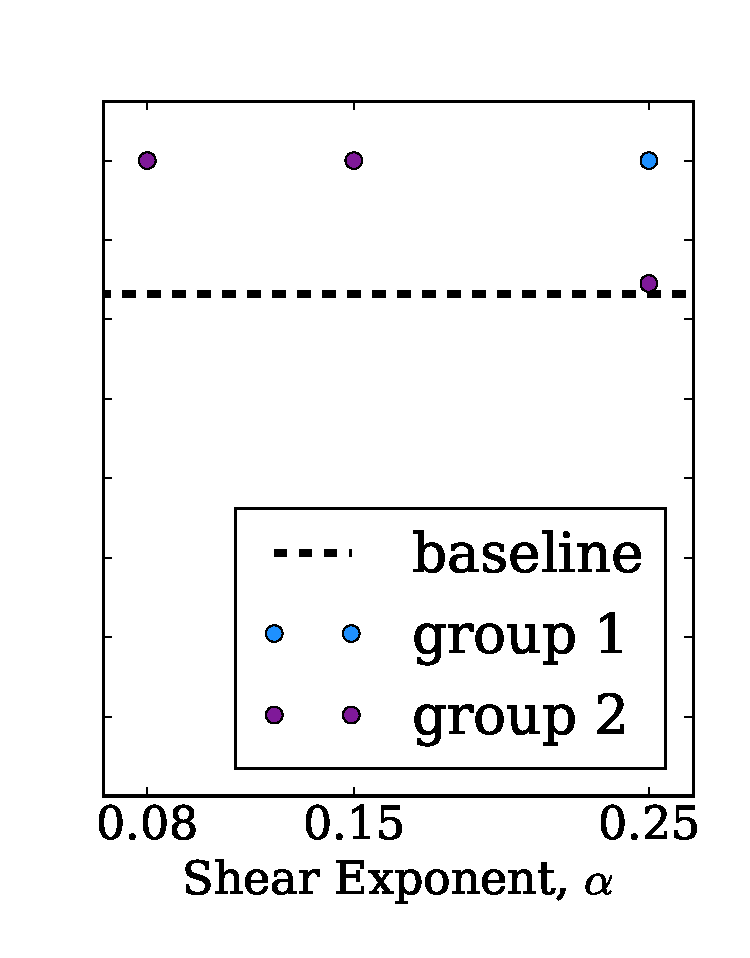
\includegraphics[width=0.25\textwidth]{D_NW_750.pdf}}\\
    \vspace{-0.25cm}
    \caption{Optimization results for the northwest dominant wind rose. The first row shows the COE, the second row shows optimal hub heights for each of the two groups, the third row shows optimal rotor diameters for each of the two groups. Each column represents a different grid spacing.}
  \label{northwest}
  \end{centering}
\end{figure}

\newpage
For each wind rose, there was a large benefit to having different heights and rotor diameters in the farm when the turbines are very close together, corresponding to the 2.37 and 3.56 diameter grid spacing. The unidirectional wind rose benefited greatly from the non-homogeneous turbine farm, while the other wind roses realized smaller benefits. 

Figure \ref{turbines} shows the turbine heights and rotor diameters for two of the optimized cases. The large difference plot shows hub heights of 155 and 61 meters, and rotor diameters 160 and 102 meters. These values are from the unidirectional optimization for the 2.37 diameter grid spacing and 0.08 wind shear exponent. Group two is much shorter and smaller than group one, resulting in low wake interference between turbines. The small difference plot shows hub heights of 150 and 80 meters and rotor diameters of 160 and 140 meters. These values are from  the northwest dominant wind rose, with 3.56 diameter grid spacing and 0.15 shear exponent. In this case there is still a difference in the turbine heights and diameters, but not as extreme. In this specific wind farm, the decreased wake interference from smaller rotor diameters is outweighed by the increased power from larger rotors and taller towers.

\begin{figure}[htbp]
\begin{centering}
	\subfloat[Heights and rotor diameters corresponding to the unidirectional wind rose, 300 meter grid spacing, and 0.08 wind shear exponent.]{\includegraphics[width=0.49\textwidth]{large_difference.pdf}}
    \subfloat[Heights and rotor diameters corresponding to the northwest dominant wind rose, 450 meter grid spacing, and 0.15 wind shear exponent.]{\includegraphics[width=0.49\textwidth]{small_difference.pdf}}
    \caption{Visual representation of different rotor heights and diameters. The figure on the left represents a large difference in rotor diameter and height, while on the right there is a smaller difference between the two groups.}
  \label{turbines}
  \end{centering}
\end{figure}



% In past research we have explored optimized two different height groups in a wind farm with constant rotor diameter \cite{Stanley2017_WE}. Figure \ref{just_heights} shows the optimized COE for the unidirectional wind rose for two cases: two different turbine groups where each group has a different hub height and rotor diameter and two different turbine groups where each group has a different hub height, but the rotor diameter is constant across the farm. For the 300 meter grid spacing there is a significantly lower COE when different rotor diameters are included in the farm, a 12\%-18\% decrease across the three shear exponents considered. The other grid spacings are also much better with different rotor diameters for the two lower shear exponents, but at the highest shear exponent of 0.25, allowing for different hub heights and rotor diameters was practically the same as just different hub heights with uniform rotor diameter. The other wind roses showed much lower COE decrease when allowing different rotor diameters and hub heights compared to just allowing different hub heights. 




% \begin{figure}[htbp]
% \begin{centering}
% 	\subfloat{\includegraphics[height=0.3\textwidth]{justHeights_300.pdf}}
%     \hspace{-0.36cm}
%     \subfloat{\includegraphics[height=0.3\textwidth]{justHeights_450.pdf}}
%     \hspace{-0.36cm}
%     \subfloat{\includegraphics[height=0.3\textwidth]{justHeights_600.pdf}}
%     \hspace{-0.36cm}
%     \subfloat{\includegraphics[height=0.3\textwidth]{justHeights_750.pdf}}\\
%     \caption{For the unidirectional wind rose, optimized COE with different hub heights and rotor diameters throughout the farm compared to optimized COE of a farm with different hub heights but homogeneous rotor diameter.}
%   \label{just_heights}
%   \end{centering}
% \end{figure}


\FloatBarrier

\section{Conclusions and Continued Development}

In this research, we explored the COE decreases associated with non-homogeneous turbine height and rotor diameter wind farms. We discussed how to model wind farm COE in non-homogeneous turbine wind farms, and optimized wind farms with different wind roses, grid spacing, and wind shear. For a unidirectional wind rose, there was a significant COE decrease in the non-homogeneous turbine wind farm compared to an identical turbine farm. Compared to the baseline, two different turbine groups achieved a COE decrease between 22.2\% and 41.5\%, while uniform turbine optimization realized between a 4.2\% and 12.8\% COE decrease. For the other wind roses, west dominant and northwest dominant, there was large benefit for two turbine groups for grid spacings of 2.37 to 3.56 diameters. The COE decrease compared to baseline was between 4.7\% and 18.8\% for two groups, and 3.4\% and 10.2\% for on group. At larger grid spacings, the COE decrease was not significant. 

These conclusions are significant in wind farm design. New wind farms can be designed with different turbine heights and rotor diameters to produce cheaper wind energy. Also, additional turbines may be built in existing farms to increase power production, without negatively affecting the already existing turbines. 

There are several ways that this research is being further developed.
\begin{itemize}
\item \textbf{Optimize complete turbine design.} In addition to hub height, rotor diameter, tower diameter, and tower thickness, other aspects of turbine design will be included in optimization. This will include rated power, drivetrain design, and blade chord and twist distributions. The goal should be to approach complete turbine design.
\item \textbf{Couple turbine design with layout and yaw control optimization.} Coupling non-homogeneous turbine design with current wake interaction minimization methods may reflect additional COE decrease benefits than when each is performed individually.
\item{\textbf{Optimize with analytic gradients.}} Analytic exact gradients allow for much better optimization convergence than finite-difference approximation. Additionally, finite-difference gradients are more computationally expensive than analytic gradients, especially as the number of design variables increases. When coupling the wind turbine design with layout optimization and yaw control, analytic gradients become a necessity. We currently have more than 90\% of the gradients for the entire wind farm model, and will optimize with exact gradients in future research.
\item{\textbf{Consider other wind roses.}} Optimizing with different wind roses will lend further insight to which situations best benefit from non-identical turbine type wind farms.
\item{\textbf{Consider discrete variables.} Differing the amount of wind turbines and changing the number of turbines in each group may both lend further understanding to the effectiveness of non-homogeneous turbine wind farms. One potential way to study this would be to assign the number of turbines in each group as a design variable and allow turbines to switch groups during optimization. However, turbine number and group designation are both discrete variables making the optimization much more challenging. We will address these discrete variables by selecting several numbers of turbines and various distributions of the different groups, and optimizing each case with the method described in this paper.}
% \item{\textbf{Consider wind farms with different amounts of wind turbines.}} Considering larger and smaller farms will help us better understand situations best suited for non-homogeneous turbine farms.
% % \item{\textbf{Consider more turbine groups.}} In this study we only consider two different turbine groups. However, three or four groups may results in significantly lower COE. Even allowing each turbine to vary individually might have large benefits.
% \item{\textbf{Consider different ratios of turbine groups.}} In this study, 13 turbines are in group one, and 12 are in group two. Other group ratios may be much more effective in reducing COE. One potential way to study this would be to assign the turbine group designation as a design variable and allow turbines to switch group during optimization. This would yield interesting results, but would no longer be gradient-based optimization as group designation is a discrete variable.
% \item{\textbf{Consider different distributions of the different turbine groups in the farm.}} In this study we assigned the different height groups in a checkerboard pattern. Alternating rows or another distribution of the height groups within the wind farm may result in lower COE.
\end{itemize}

% This research will be continued by including other aspects of turbine design as design variables in optimization, with the goal to approach complete turbine design. This will include turbine rating, aspects of the drivetrain, and blade design. Including coupled turbine layout, and potentially yaw control optimization will add more insight into the benefits of non-homogeneous turbine wind farms.

% Additionally, analytic gradients will be used across the entire model, accelerating the optimization process and allowing better convergence. Along with more wind roses, different wind farm boundaries should also be explored, as well as changing the total number of turbines. Another major development should be to research changing the ratio of turbines in each group, along with their distribution in the wind farm. This could be achieved by intelligently selecting different ratios and distributions in the wind farm and optimizing individually, or possibly including the group designation as a design variable (however this would no longer allow gradient-based optimization as group designation is discrete). Finally, exploring additional turbine groups will lend further understanding and possibly uncover additional benefits of non-homogeneous turbine wind farms.  

\section*{Acknowledgments}
The BYU authors developed this journal article based on funding from the Alliance for Sustainable Energy, LLC, Managing and Operating Contractor for the National Renewable Energy Laboratory for the U.S. Department of Energy.  The NREL authors were supported by the U.S. Department of Energy (DOE) under Contract No. DE-AC36-08GO28308 with the National Renewable Energy Laboratory.

Funding for the work was provided by the DOE Office of Energy Efficiency and Renewable Energy, Wind Energy Technologies Office.

The U.S. Government retains and the publisher, by accepting the article for publication, acknowledges that the U.S. Government retains a nonexclusive, paid-up, irrevocable, worldwide license to publish or reproduce the published form of this work, or allow others to do so, for U.S. Government purposes.

\bibliography{references}

% \begin{table}
% \caption{\label{tab:table1} Transitions selected for thermometry}
% \centering
% \begin{tabular}{lcccccc}
% \hline
% & Transition& & \multicolumn{2}{c}{}\\\cline{2-2}
% Line& $\nu''$& & $J'' $& Frequency, cm$^{-1}$& $FJ$, cm$^{-1}$& $G\nu $, cm$^{-1}$\\\hline
% a& 0& P$_{12}$& 2.5& 44069.416& 73.58& 948.66\\
% b& 1& R$_{2}$& 2.5& 42229.348& 73.41& 2824.76\\
% c& 2& R$_{21}$& 805& 40562.179& 71.37& 4672.68\\
% d& 0& R$_{2}$& 23.5& 42516.527& 1045.85& 948.76\\
% \hline
% \end{tabular}
% \end{table}

\end{document}
